% ============================================================
% main.tex  --  Single-column journal manuscript
% Compile: pdflatex main; bibtex main; pdflatex main; pdflatex main
% ============================================================
\documentclass[11pt,a4paper]{article}
\usepackage[T1]{fontenc}
\usepackage[a4paper,margin=2.2cm]{geometry}
\usepackage{amsmath,amssymb,amsfonts}
\usepackage{graphicx}
\graphicspath{{figures/}}
\usepackage{textcomp}
\usepackage{xcolor}
\usepackage{cite}
\usepackage[hyphens]{url}
\def\UrlBreaks{\do\/\do\-\do\.\do\_\do\=\do\?\do\&}
\Urlmuskip=0mu plus 2mu
\usepackage{caption}
\captionsetup{font=small,labelfont=bf}
\linespread{1.08}
\setlength{\parskip}{3pt}
\setlength{\emergencystretch}{3em}
\renewcommand{\topfraction}{0.9}\renewcommand{\bottomfraction}{0.9}
\renewcommand{\textfraction}{0.08}\renewcommand{\floatpagefraction}{0.75}
\newcommand{\figref}[1]{Fig.~\ref{fig:#1}}
\newcommand{\todo}[1]{\textcolor{red}{#1}}% red = confirm or fill before submission
\providecommand{\PARstart}[2]{#1#2}
\newcommand{\appendices}{\appendix}
\newcommand{\nSurvey}{43}
\newcommand{\nLA}{22}
\newcommand{\shareLA}{51.2}
\newcommand{\costMedLA}{29{,}000}
\newcommand{\costMeanLA}{46{,}318}
\newcommand{\replMedLA}{18}
\newcommand{\replNLA}{21}
\newcommand{\replMeanLA}{22.0}
\newcommand{\kmMeanLA}{83.0}
\newcommand{\resaleRatioLA}{43}
\newcommand{\resaleMedLA}{42}
\newcommand{\ageMeanLA}{14.1}
\newcommand{\nbMeanLA}{4.5}
\newcommand{\nLFP}{5}
\newcommand{\shareLFP}{11.6}
\newcommand{\costMedLFP}{100{,}000}
\newcommand{\costMeanLFP}{105{,}400}
\newcommand{\replMedLFP}{43.5}
\newcommand{\replNLFP}{4}
\newcommand{\replMeanLFP}{42.8}
\newcommand{\kmMeanLFP}{106.2}
\newcommand{\resaleRatioLFP}{13}
\newcommand{\resaleMedLFP}{16}
\newcommand{\ageMeanLFP}{18.4}
\newcommand{\nbMeanLFP}{2.8}
\newcommand{\nPW}{16}
\newcommand{\sharePW}{37.2}
\newcommand{\costMedPW}{28{,}000}
\newcommand{\costMeanPW}{32{,}906}
\newcommand{\replMedPW}{30}
\newcommand{\replNPW}{16}
\newcommand{\replMeanPW}{29.2}
\newcommand{\kmMeanPW}{56.9}
\newcommand{\resaleRatioPW}{36}
\newcommand{\resaleMedPW}{37}
\newcommand{\ageMeanPW}{21.0}
\newcommand{\nbMeanPW}{4.4}
\newcommand{\kmAll}{76}
\newcommand{\costRatio}{3.4}
\newcommand{\rangeShare}{72.1}
\newcommand{\rangeN}{31}
\newcommand{\nAgeA}{13}
\newcommand{\rngAgeA}{46}
\newcommand{\nAgeB}{10}
\newcommand{\rngAgeB}{80}
\newcommand{\nAgeC}{20}
\newcommand{\rngAgeC}{85}
\newcommand{\onePerDay}{42}
\newcommand{\fourBat}{31}
\newcommand{\fourBatLA}{15}
\newcommand{\ciLAlo}{17.5}
\newcommand{\ciLAhi}{30.0}
\newcommand{\ciLFPlo}{30.0}
\newcommand{\ciLFPhi}{54.0}
\newcommand{\replMinLA}{8}
\newcommand{\replMaxLA}{30}
\newcommand{\replMinLFP}{30}
\newcommand{\replMaxLFP}{54}
\newcommand{\replLAnobatch}{16.2}
\newcommand{\nLAnobatch}{12}
\newcommand{\ahMed}{140}
\newcommand{\ahN}{4}
\newcommand{\packKWh}{6.7}
\newcommand{\kmUsed}{76}
\newcommand{\ekmUsed}{71.4}
\newcommand{\speedUsed}{16.8}
\newcommand{\NcalLA}{920}
\newcommand{\NcalLFP}{1{,}540}
\newcommand{\priceLA}{29{,}000}
\newcommand{\priceLFP}{100{,}000}
\newcommand{\scrapLA}{42}
\newcommand{\scrapLFP}{16}
\newcommand{\lifeLA}{18.0}
\newcommand{\tcoLA}{245{,}912}
\newcommand{\effLA}{90.1}
\newcommand{\egLA}{8.37}
\newcommand{\cpkLA}{1.91}
\newcommand{\dodLA}{88}
\newcommand{\dodmaxLA}{97}
\newcommand{\rngLA}{69}
\newcommand{\repLA}{6}
\newcommand{\tcoFiveLA}{157{,}551}
\newcommand{\lifeLFP}{43.5}
\newcommand{\tcoLFP}{322{,}226}
\newcommand{\effLFP}{97.8}
\newcommand{\egLFP}{7.09}
\newcommand{\cpkLFP}{2.50}
\newcommand{\dodLFP}{82}
\newcommand{\dodmaxLFP}{85}
\newcommand{\rngLFP}{74}
\newcommand{\repLFP}{2}
\newcommand{\tcoFiveLFP}{207{,}967}
\newcommand{\gapLFP}{76{,}315}
\newcommand{\gapPct}{31}
\newcommand{\gridratio}{15.2}
\newcommand{\TcellK}{30.8}
\newcommand{\Tspread}{0.32}
\newcommand{\TcKhulna}{30.8}
\newcommand{\TcChuadanga}{30.8}
\newcommand{\TcRajshahi}{30.5}
\newcommand{\TannKhulnaAtwofour}{25.97}
\newcommand{\TannChuadangaAtwofour}{26.10}
\newcommand{\TannRajshahiAtwofour}{25.71}
\newcommand{\TannKhulnaBtwofive}{25.59}
\newcommand{\TannChuadangaBtwofive}{25.50}
\newcommand{\TannRajshahiBtwofive}{25.23}
\newcommand{\Tmin}{15.5}
\newcommand{\Tmax}{33.6}
\newcommand{\lifeLAKhulna}{18.0}
\newcommand{\lifeLFPKhulna}{43.5}
\newcommand{\lifeLAChuadanga}{17.8}
\newcommand{\lifeLFPChuadanga}{43.3}
\newcommand{\lifeLARajshahi}{18.1}
\newcommand{\lifeLFPRajshahi}{43.7}
\newcommand{\litLifeLA}{7.8}
\newcommand{\litLifeLFP}{70.6}
\newcommand{\litErrLA}{-57}
\newcommand{\litErrLAabs}{57}
\newcommand{\litErrLFP}{62}
\newcommand{\litGap}{61{,}413}
\newcommand{\heatLA}{3.4}
\newcommand{\heatLFP}{2.0}
\newcommand{\vEgrid}{8.4}
\newcommand{\vClean}{9.6}
\newcommand{\vCleanPct}{13}
\newcommand{\vUnctad}{9.2}
\newcommand{\vUnctadPct}{9}
\newcommand{\beP}{58{,}622}
\newcommand{\bePpct}{41}
\newcommand{\beL}{98}
\newcommand{\bePA}{43{,}876}
\newcommand{\bePB}{69{,}615}
\newcommand{\bePC}{82{,}304}
\newcommand{\bePD}{98{,}869}
\newcommand{\premium}{71{,}000}
\newcommand{\extFav}{-147{,}457}
\newcommand{\extUnfav}{245{,}143}
\newcommand{\laEightGap}{-8{,}833}
\newcommand{\laThirtyGap}{102{,}440}
\newcommand{\perbikeLA}{1{,}736}
\newcommand{\packsLA}{0.67}
\newcommand{\opLA}{1{,}556}
\newcommand{\embLA}{180}
\newcommand{\perbikeLFP}{1{,}412}
\newcommand{\packsLFP}{0.28}
\newcommand{\opLFP}{1{,}319}
\newcommand{\embLFP}{93}
\newcommand{\saveBike}{324}
\newcommand{\saveOp}{237}
\newcommand{\saveEmb}{87}
\newcommand{\fleetA}{0.45}
\newcommand{\fleetB}{0.97}
\newcommand{\fleetOpA}{0.33}
\newcommand{\fleetEmbA}{0.12}
\newcommand{\leadLow}{52}
\newcommand{\leadMid}{79}
\newcommand{\leadHigh}{117}
\newcommand{\leadBikeLow}{37}
\newcommand{\leadBikeHigh}{84}
\newcommand{\abateCarbon}{23{,}560}
\newcommand{\abateLead}{136}
\newcommand{\abateLeadLow}{91}
\newcommand{\abateLeadHigh}{204}
\newcommand{\suppFull}{107}
\newcommand{\suppHalf}{53}
\newcommand{\polFullCO}{0.45}
\newcommand{\polHalfCO}{0.23}
\newcommand{\sensMin}{186}
\newcommand{\sensMax}{354}
\newcommand{\tarLow}{84{,}572}
\newcommand{\tarHigh}{66{,}256}
\newcommand{\EFgrid}{0.62}
% every number used in the text is defined here
% ============================================================
% title_block.tex  --  Title and author information
% ============================================================
\title{%
When Does Lithium Replace Lead?\\
A Survey-Calibrated, Temperature-Driven Assessment of Cost,\\
Carbon and Lead Flow for Easy-Bike Batteries in Bangladesh%
}

\author{%
    Razowan Kabir$^{1,*}$,
    \todo{Md. Raju Mridha}$^{1}$,
    \todo{Meshkat Sorif}$^{2}$,
    and \todo{Md Atikur Rahman}$^{1}$%
    \\[6pt]
    \parbox{0.92\textwidth}{\centering\small
        $^{1}$Department of Electrical and Electronic Engineering,
        Khulna University of Engineering and Technology,
        Khulna, Bangladesh\\[2pt]
        $^{2}$\todo{Department of Electrical and Electronic Engineering, Gopalganj Science and Technology University},
        \todo{Gopalganj, Bangladesh}\\[2pt]
        $^{*}$Corresponding author:
        \todo{rkrazowan@gmail.com};
        ORCID: \todo{0009-0008-6274-8117}%
    }%
}
\date{Draft, October 2026}

\begin{document}
\maketitle
\begin{abstract}
Electric easy-bikes carry much of Bangladesh's short-distance transport, yet most run on lead-acid batteries that last about \lifeLA{} months and feed an informal recycling chain that is a leading source of lead exposure. Whether lithium iron phosphate (LFP) packs should replace them depends on field cost and life, not on laboratory cycle life alone. We combine a field survey of \nSurvey{} easy-bike drivers (October 2026) with NASA POWER temperature for Khulna, Chuadanga and Rajshahi (2024--2025) in a MATLAB/Simulink model of capacity, resistance, depth of discharge, Arrhenius ageing, replacement-aware cost, carbon and lead flow. Survey prices (median BDT \costMedLA{} lead-acid, \costMedLFP{} LFP), replacement intervals (\replMedLA{} and \replMedLFP{} months), resale values and daily distance (\kmAll{} km) replace literature assumptions, and the model is checked against the survey and published energy per charge. Literature cycle lives would make LFP BDT \litGap{} cheaper over ten years, but survey-anchored lives make it BDT \gapLFP{} (\gapPct\%) dearer for the operator. LFP breaks even at a set price of about BDT \beP{} or a life of about \beL{} months. It still cuts grid electricity by \gridratio\%, saves about \saveBike{} kg CO$_2$e per bike-year and removes \leadLow--\leadHigh{} kt of lead per year from recycling at 1.4 million bikes, at an implied BDT \abateCarbon{} per tonne CO$_2$e. Mean battery temperatures at the three sites differ by only \Tspread\,$^\circ$C, so site does not change the ranking. The survey is a small convenience sample and the LFP results rest on five drivers.
\end{abstract}
\noindent\textbf{Keywords:} easy-bike; lead-acid battery; lithium iron phosphate; field survey; NASA POWER; battery degradation; total cost of ownership; carbon emissions; lead pollution; Bangladesh
\bigskip

\section{Introduction}
\label{sec:intro}
Battery-powered three-wheelers (easy-bikes, Mishuks, e-rickshaws) have become a mass transport mode in Bangladesh. A CLEAN/BWGED study estimates about 1.4 million easy-bikes consuming roughly 4{,}905 GWh of electricity per year \cite{clean2024}, whereas Pure Earth puts the number of electric three-wheelers at 3--4 million \cite{pureearth_smep}; we treat both as scenarios. Lead-acid batteries dominate \cite{mordor2026} and are short-lived: a battery set costing more than BDT 72{,}000 is reported to last 8--11 months \cite{fe2024}, and a 2026 field study of 150 drivers in Gopalganj and Khulna documents prolonged hub charging, frequent overloading and lead-acid degradation \cite{chowdhury2026}.

This short life has three consequences. First, replacement is a large part of operator cost. Second, internal resistance and charger losses waste electricity, and each replacement carries manufacturing emissions. Third, used lead-acid batteries (ULABs) are broken and smelted largely by the informal sector, a primary contributor to lead-pollution hotspots \cite{esdo2021}. The national public-health bulletin of IEDCR reports that about 36 million Bangladeshi children (60\%) are poisoned by lead and, citing a World Bank study in The Lancet, that lead causes a loss of about 20 million IQ points and 140{,}000 cardiovascular deaths in adults; the 2019 economic burden was US\$28.6 billion, or 6--9\% of GDP \cite{das2026}. Pure Earth reports about 125 kg of lead in one easy-bike's batteries and about 167{,}000 t of lead waste per year from recycling them \cite{fe2024,pureearth_smep}.

LFP batteries offer higher round-trip efficiency, longer cycle life and no lead, but cost more. Laboratory cycle-life figures suggest they should be cheaper over a bike's life; whether drivers' actual prices and replacement intervals support this is an empirical question. Bangladesh is also hot: monthly mean 2\,m temperature in the study area ranges from \Tmin\ to \Tmax\,$^\circ$C (\figref{temp}), and a 42\,$^\circ$C day has been reported at Chuadanga \cite{heat2025}. Heat accelerates ageing of every chemistry, but not equally.

\textbf{Research gap.} Existing work compares lead-acid and lithium-ion for stationary storage \cite{keshan2016,yudhistira2022,jasper2025}, studies cell ageing \cite{yagci2026}, thermal safety \cite{schoberl2024}, charging infrastructure \cite{hasan2020}, or easy-bike operation and energy use for lead-acid only \cite{chowdhury2026,peakdemand}. In web searches of publisher and data sites in October 2026 we found no study that anchors a temperature-driven chemistry comparison for Bangladesh easy-bikes on drivers' own purchase prices, replacement intervals and resale values, and that adds carbon and lead-flow accounting. \todo{[State the databases, search terms and dates of your final literature search.]}

\textbf{Contributions.} (i) A field survey of \nSurvey{} drivers (October 2026) whose cleaned data supply the cost, life, resale and distance inputs. (ii) A reproducible MATLAB/Simulink model, driven by NASA POWER temperature, with analytic and block-diagram versions cross-checked. (iii) A calibration and validation design that exposes how far laboratory cycle lives are from field practice (\figref{validlife}). (iv) Break-even price and life for LFP, sensitivity, carbon and lead-flow accounting, and the operator support implied by conversion scenarios.

Section~\ref{sec:data} reviews the literature and inputs, Section~\ref{sec:method} describes the survey and model, Section~\ref{sec:results} gives results, Section~\ref{sec:disc} discusses implications and limits, and Section~\ref{sec:concl} concludes.

\section{Literature and Input Data}
\label{sec:data}
\subsection{Literature used}
Table~\ref{tab:lit} lists the published sources and what each contributes. Entries marked $\dagger$ were supplied in the author's data file; their ranges are used as stated and only for the round-trip efficiency and the literature cycle life used for comparison.
\begin{table}[t]
\caption{Literature used, the finding relevant to this work, and the gap it leaves.}
\label{tab:lit}
\centering\footnotesize
\renewcommand{\arraystretch}{1.1}
\begin{tabular}{p{2.6cm}p{3.0cm}p{6.0cm}p{2.8cm}}
\hline
Source & Scope & Finding used here & Gap addressed here \\
\hline
Chowdhury \emph{et al.} \cite{chowdhury2026} & Field survey ($n$=150, Gopalganj and Khulna) and one instrumented bike & Lead-acid banks; 8--9 kWh per full charge; about 20 A at 60 V with five passengers; iron-core chargers about 80\%; hub fee BDT 80--100 per charge & Lead-acid only; no chemistry or temperature model \\
CLEAN/BWGED \cite{clean2024} & Fleet and grid load & about 1.4 M bikes; about 4{,}905 GWh/yr & Fleet level only \\
Pure Earth \cite{pureearth_smep,fe2024}; IEDCR \cite{das2026}; UNCTAD \cite{unctad_smep} & ULAB policy and lead burden & 3--4 M electric three-wheelers; about 125 kg Pb per easy-bike; 167{,}000 t Pb waste per year; 36 M children poisoned; about 80\% of ULAB recycled informally & Not linked to battery life or chemistry \\
Hasan \cite{hasan2020} & E-rickshaw charging stations & Packs of four 150 Ah, 12 V batteries (7.2 kWh); charging efficiency 89\% & Lead-acid only \\
Yagci \emph{et al.} \cite{yagci2026} & LFP ageing & $E_a$ = 37.3 $\pm$ 12.8 kJ/mol & Stationary cells \\
Tsujikawa \emph{et al.} \cite{tsujikawa2009}; \cite{bu806a} & VRLA ageing & Life roughly halves per 8--10\,$^\circ$C; damage summed over variable temperature & Float service \\
Jasper \emph{et al.} \cite{jasper2025}; Yudhistira \emph{et al.} \cite{yudhistira2022} & Life-cycle assessment & Production and end of life about 40 kg CO$_2$e/kWh for lead-acid; LFP lower impact per kWh delivered where many cycles occur & European data; not easy-bike duty \\
Keshan \emph{et al.} \cite{keshan2016}$\dagger$ & Off-grid stationary storage & Efficiency and cycle-life ranges (400 and 2{,}500 cycles used only as the literature comparison) & Stationary, not traction \\
Sch\"oberl \emph{et al.} \cite{schoberl2024} & Thermal runaway & Graphite/NMC-811 needs significantly higher safety measures than graphite/LFP & Safety only \\
Chowdhury \emph{et al.} \cite{chowdhury2021}; \cite{eos2026} & Remediation near ULAB sites & Soil lead $-$96\%, child blood lead $-$35\% (Savar); $-$22\% (Tangail) & Health only \\
This study's survey \cite{survey2026} & $n$=43 drivers, October 2026 & Purchase price, set size, daily distance, replacement interval, resale value, main problem & Convenience sample; LFP $n$=5 \\
\hline
\end{tabular}
\end{table}

\subsection{Parameter matrix}
Tables~\ref{tab:params1} and \ref{tab:params2} list every model input, its value, source and status: \emph{Survey} (taken from the field survey, Section~\ref{sec:survey}), \emph{Sourced} (published or official), \emph{Derived} (computed from the two), \emph{Calibrated} (fitted to the survey) or \emph{Scenario} (no source found; varied in Section~\ref{sec:sens}). LA = lead-acid; values are listed as LA / LFP where they differ.
\begin{table}[t]
\caption{Parameter matrix, part 1: pack, performance and temperature effects.}
\label{tab:params1}
\centering\footnotesize
\renewcommand{\arraystretch}{1.1}
\begin{tabular}{p{2.5cm}p{3.3cm}p{6.8cm}p{1.8cm}}
\hline
Parameter & Model value & Source / reason & Status \\
\hline
Pack voltage & 48 / 48 V & Four 12 V batteries per set is the most common configuration (\fourBat{} of \nSurvey{} respondents; \fourBatLA{} of \nLA{} lead-acid); LFP users reported 48 V & Survey \\
Pack capacity & \ahMed{} / \ahMed{} Ah (\packKWh{} kWh) & Median of the four lead-acid capacities reported (120, 120, 160, 180 Ah; a fifth value of 30 Ah looks like a charger current and is excluded); LFP capacity was not reported and is set equal & Survey, derived \\
Round-trip efficiency & 77.5 / 95\% & Midpoints of ranges in the author's data file \cite{keshan2016} & Sourced$\dagger$ \\
Cycle life $N_{80}$ at 80\% DoD, 25\,$^\circ$C & \NcalLA{} / \NcalLFP{} cycles & Fitted so that modelled life at Khulna equals the survey median replacement interval (\replMedLA{} / \replMedLFP{} months); literature values 400 / 2{,}500 \cite{keshan2016} are shown for comparison & Calibrated \\
Set price (BDT) & \priceLA{} / \priceLFP{} & Median purchase price of the current set (survey, $n$ = \nLA{} / \nLFP{}) & Survey \\
Resale of old set & \scrapLA{} / \scrapLFP{}\% of price & Median of individual resale/purchase ratios & Survey \\
Ambient temperature & 15.5--33.6\,$^\circ$C monthly mean & NASA POWER T2M, MERRA-2 \cite{nasa_power,gelaro2017}; 42\,$^\circ$C day \cite{heat2025} & Sourced \\
LA life vs heat & Halves per 8 K above 25\,$^\circ$C & \cite{bu806a}; peer-reviewed 10 K \cite{tsujikawa2009} tested in Section~\ref{sec:sens} & Sourced \\
LFP ageing $E_a$ & 37.3 kJ/mol & 37.3 $\pm$ 12.8 \cite{yagci2026} & Sourced \\
Capacity factor vs $T$ (0, 10, 25, 40, 50\,$^\circ$C) & LA 0.84, 0.90, 1.00, 1.05, 1.05; LFP 0.79, 0.91, 1.00, 1.02, 1.02 & Vendor notes: LA \cite{discoverbattery}; LFP above 25\,$^\circ$C \cite{bonnen2026}, cold side supported qualitatively by \cite{bauknecht2023}. Only months below 25\,$^\circ$C are affected & Vendor-level \\
Resistance sensitivity $E_r$ & 25 / 20 kJ/mol & No source found; small effect & Scenario \\
Cycle-life DoD exponent $k$ & 1.4 / 1.0 & No source found; cycle life $\propto (0.8/\mathrm{DoD})^k$ & Scenario \\
Battery above ambient & +5\,$^\circ$C (0 and 10 tested) & Not measured in the survey or in \cite{chowdhury2026}; a large uncertainty & Scenario \\
\hline
\end{tabular}
\end{table}
\begin{table}[t]
\caption{Parameter matrix, part 2: duty cycle, economics, fleet, carbon and lead.}
\label{tab:params2}
\centering\footnotesize
\renewcommand{\arraystretch}{1.1}
\begin{tabular}{p{2.5cm}p{3.3cm}p{6.8cm}p{1.8cm}}
\hline
Parameter & Model value & Source / reason & Status \\
\hline
Daily distance & \kmUsed{} km (50--100 tested) & Mean of all \nSurvey{} respondents (lead-acid \kmMeanLA{}, LFP \kmMeanLFP{}, Powder \kmMeanPW{} km) & Survey \\
Charges per day & 1 & \onePerDay{} of \nSurvey{} drivers charge once a day & Survey \\
Energy use & \ekmUsed{} Wh/km (52--88 tested) & Lower of two published values (71.4 and 88 Wh/km) cited in \cite{peakdemand}; consistent with a \packKWh{} kWh set serving about 83 km at about 90\% DoD & Sourced \\
Average speed & \speedUsed{} km/h & 1.2 kW (20 A $\times$ 60 V, five passengers \cite{chowdhury2026}) divided by the energy use & Derived \\
Charger efficiency & 80\% & Iron-core chargers \cite{chowdhury2026}; 89\% reported for e-rickshaw stations \cite{hasan2020} & Sourced \\
Operating days & 300 per year (250--350 tested) & Not asked in the survey; absorbed in the calibrated cycle life & Scenario \\
Tariff & BDT 11.36/kWh (7.70 and 16.24 tested) & BERC order of June 3, 2026, battery/EV-charging category \cite{berc2026fe,fenews2026}; hub-fee check: BDT 80--100 per 8--9 kWh $\approx$ 10.6 \cite{chowdhury2026} & Sourced (press) \\
Discount rate & 11.96\% ($\pm$20\% tested) & Weighted-average lending rate on advances, April 2026 \cite{ceic_lending} & Sourced \\
Maintenance & 0 & No source found; battery-only cost & Scenario \\
Fleet size & 1.4 M \cite{clean2024}; 3.0 M & Sources disagree (3--4 M \cite{pureearth_smep}; about 4 M and 500{,}000 autorickshaws \cite{unctad_smep}) & Sourced \\
Grid emission factor & 0.62 tCO$_2$/MWh (0.55--0.70 tested) & Department of Environment, 2020--22 \cite{doe_gef} & Sourced \\
Manufacture and EOL carbon & 40 / 50 kg CO$_2$e/kWh (LFP 50--110 tested) & \cite{jasper2025}; European study & Sourced \\
Lead per set & 56 / 84 / 125 kg & Four batteries of 14--21 kg lead each \cite{smep2024}; 125 kg per easy-bike \cite{fe2024,pureearth_smep} & Sourced, scenario \\
Informal recycling share & 70--80\% & Only 30\% of ULAB recycling is formal \cite{fe2024}; about 80\% informal \cite{unctad_smep} & Sourced \\
\hline
\end{tabular}
\end{table}

\section{Methodology}
\label{sec:method}
\begin{figure}[t]
\centering
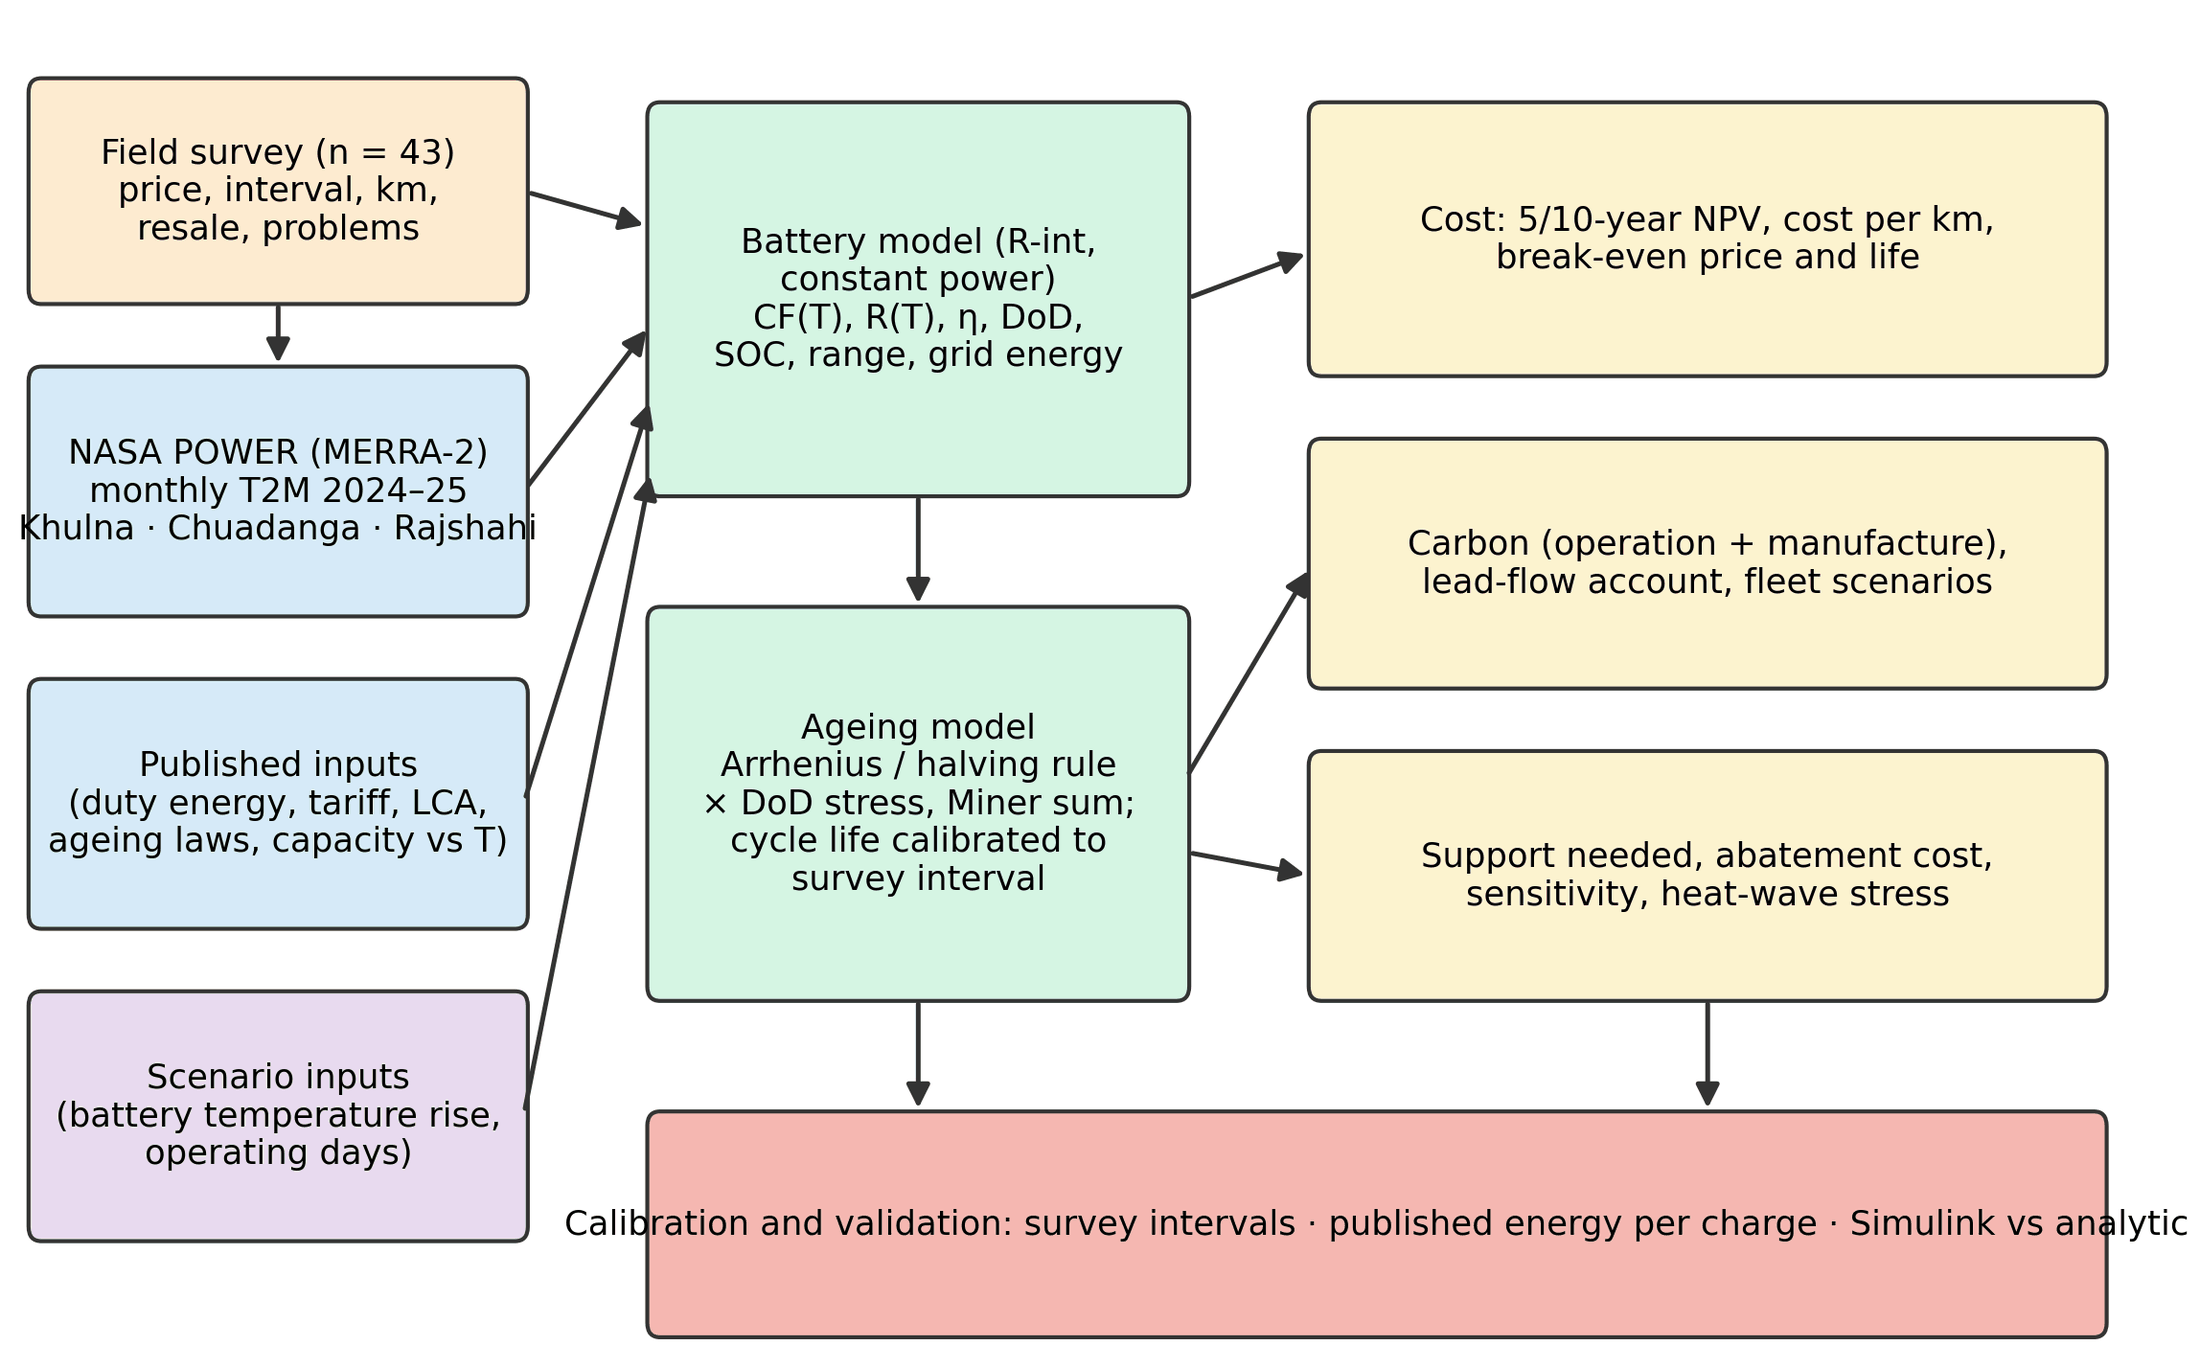
\includegraphics[width=\textwidth]{fig_method.png}
\caption{Methodology: survey, temperature, published and scenario inputs drive the battery and ageing models; outputs feed the cost, carbon, lead and policy modules; calibration and validation close the loop.}
\label{fig:method}
\end{figure}
\subsection{Study design and sites}
Three south-western sites are used for temperature: Khulna (22.84$^\circ$N, 89.57$^\circ$E), Chuadanga (23.64$^\circ$N, 88.69$^\circ$E) and Rajshahi (24.38$^\circ$N, 88.60$^\circ$E) (\figref{map}). The survey was carried out in the Khulna region (\todo{[insert district and upazila names]}), so Khulna is the calibration site; the other two sites are extrapolations through temperature only. Chuadanga was added as a heat-stress site because a 42\,$^\circ$C day was reported there in May 2025 \cite{heat2025}; in the NASA monthly means its annual mean in 2025 (\TannChuadangaBtwofive\,$^\circ$C) is not higher than Khulna's (\TannKhulnaBtwofive\,$^\circ$C), so its selection rests on peak heat, not on the mean. Two chemistries are modelled: lead-acid (LA) and LFP, the only lithium type reported in the survey.
\begin{figure}[t]
\centering
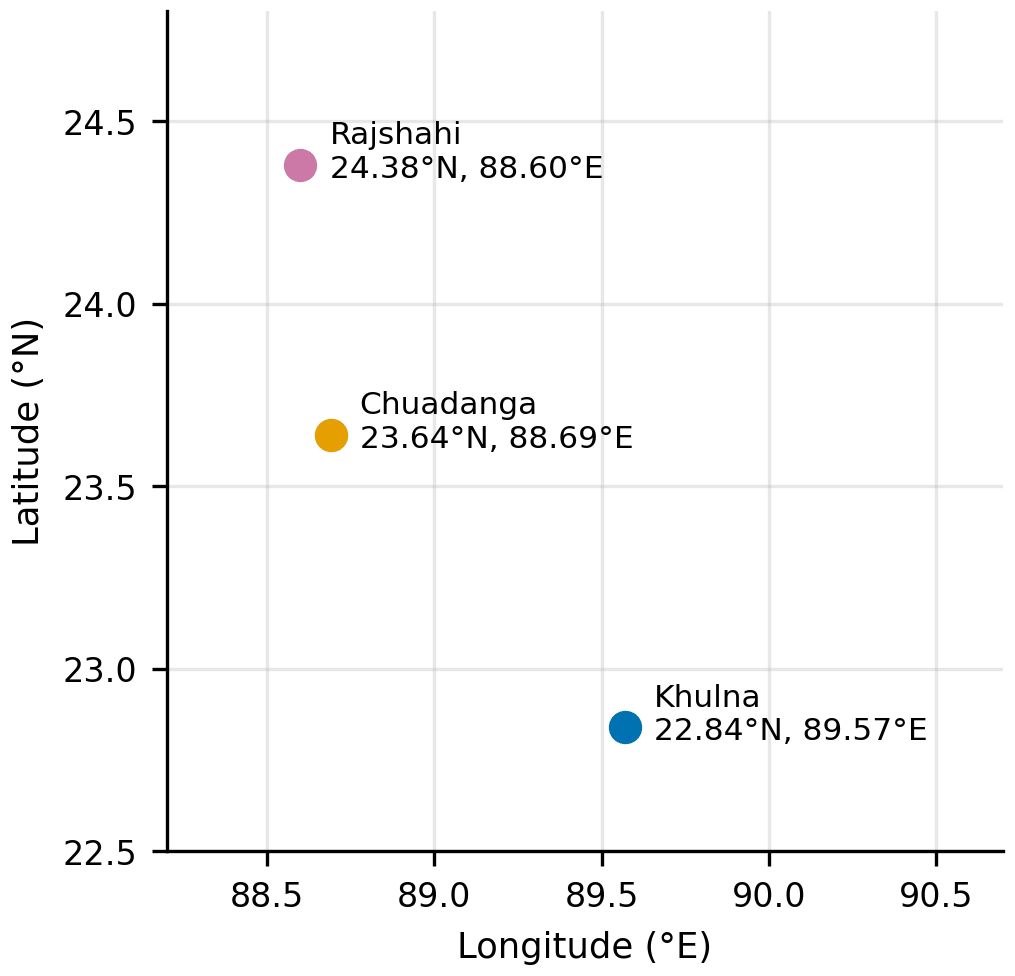
\includegraphics[width=0.5\textwidth]{fig_map.png}
\caption{NASA POWER grid points used (schematic locator).}
\label{fig:map}
\end{figure}

\subsection{Field survey}
\label{sec:survey}
Data come from a Bengali-language Google Forms questionnaire, ``Field Survey on Easy-Bike/E-Rickshaw Battery Use in Bangladesh'' \cite{survey2026}, with ten questions covering battery type, purchase cost, battery configuration, daily distance, charging frequency and cost, months in use, replacement interval, main problem and resale value. It recorded \nSurvey{} responses between 8 and 28 October 2026 from current drivers. The sample is a convenience sample, so the results are descriptive. \todo{[State ethical approval or consent procedure, and the survey locations.]}

Raw answers mixed Bengali and Western digits, ``k'' suffixes, ranges and units. Each field was converted to one unit; ``k'' was read as thousands of taka, ranges were represented by their mid-points, and the original sheet was kept unchanged. Interpreted values were flagged in a review-notes column (Appendix~\ref{app:survey}). Table~\ref{tab:use} shows which survey fields enter the model and which were deliberately not used.
\begin{table}[t]
\caption{Use of survey data in the model.}
\label{tab:use}
\centering\footnotesize
\renewcommand{\arraystretch}{1.1}
\begin{tabular}{p{3.6cm}p{5.0cm}p{6.0cm}}
\hline
Survey field & Use & Note \\
\hline
Purchase cost of current set & Initial and replacement cost $C_0$ (median by type) & LA: \nLA{}; LFP: \nLFP{} respondents; seven lead-based entries of BDT 60{,}000 or more are flagged and handled by using medians \\
Replacement interval & Calibrates $N_{80}$ (Khulna) and validates the model & LA $n$ = \replNLA{}; LFP $n$ = \replNLFP{}; LFP answers are expectations because the sets are on average \ageMeanLFP{} months old \\
Daily distance & Duty $d$ & Mean of all respondents \\
Resale value of old set & Scrap fraction $s$ & Median resale/purchase ratio by type \\
Batteries per set; Ah per battery & Pack voltage and capacity & Ah reported by only four lead-acid respondents \\
Charges per day & $n_{cyc}$ = 1 & \onePerDay{} of \nSurvey{} charge once \\
Main problem; months in use & Qualitative check of ageing-limited life & Not a model input \\
Charging cost & \emph{Not used} & Answers mix per-charge, per-month and unspecified bases and are not comparable \\
``Powder'' batteries & \emph{Not modelled} & Chemistry not confirmed; reported separately (\nPW{} respondents) \\
\hline
\end{tabular}
\end{table}

\subsection{Temperature data}
Monthly mean 2\,m air temperature (T2M, MERRA-2 \cite{gelaro2017}) for January 2024 to December 2025 was downloaded from NASA POWER \cite{nasa_power}: 24 values per site, none missing. The native grid cell is $0.5^\circ\times0.625^\circ$ (about 50--70 km), so the three points lie in neighbouring cells and are expected to be similar. Battery temperature is ambient plus $\Delta T_{op}=5\,^\circ$C, a scenario tested at 0 and 10\,$^\circ$C. Monthly means understate daily peaks (Section~\ref{sec:limits}).

\subsection{Battery model}
Each pack is a resistive (R-int) battery with temperature-dependent capacity and resistance, discharged at constant average power $P_w=e_{km}v$, where $e_{km}$ is the energy use per km and $v$ the average speed. With pack voltage $V$ and round-trip efficiency $\eta_{RT}$, the 25\,$^\circ$C resistance is chosen so that the discharge efficiency equals $\sqrt{\eta_{RT}}$ at 25\,$^\circ$C:
\begin{align}
R_{25}&=\frac{(1-\sqrt{\eta_{RT}})\sqrt{\eta_{RT}}\,V^{2}}{P_w},\\
R(T)&=R_{25}\exp\!\left[\frac{E_r}{R_g}\!\left(\frac1{T_K}-\frac1{298.15}\right)\right],\\
I&=\frac{V-\sqrt{V^{2}-4R(T)P_w}}{2R(T)},\qquad
\eta_d=1-\frac{I\,R(T)}{V}.
\end{align}
The capacity factor $CF(T)$ is interpolated from a table, so the available energy is $E_{cap}=V\,Ah\,CF(T)/1000$ kWh. With daily delivered energy $E_{day}=d\,e_{km}/1000$ for distance $d$,
\begin{align}
\mathrm{DoD}&=\frac{E_{day}}{\eta_d\,E_{cap}},\qquad
\mathrm{SOC}_{end}=\max(0,1-\mathrm{DoD}),\\
E_{grid}&=\frac{E_{day}}{\eta_d^{2}\,\eta_{chg}},\qquad
\mathrm{Range}=\frac{\mathrm{DoD}_{max}\,E_{cap}\,\eta_d}{e_{km}/1000}.
\end{align}
The same equations are implemented as a Simulink model built from core blocks (\figref{simulink}). It is run at 15, 25, 35 and 45\,$^\circ$C for both chemistries and compared with the analytic code (Appendix~\ref{app:sim}).
\begin{figure}[t]
\centering
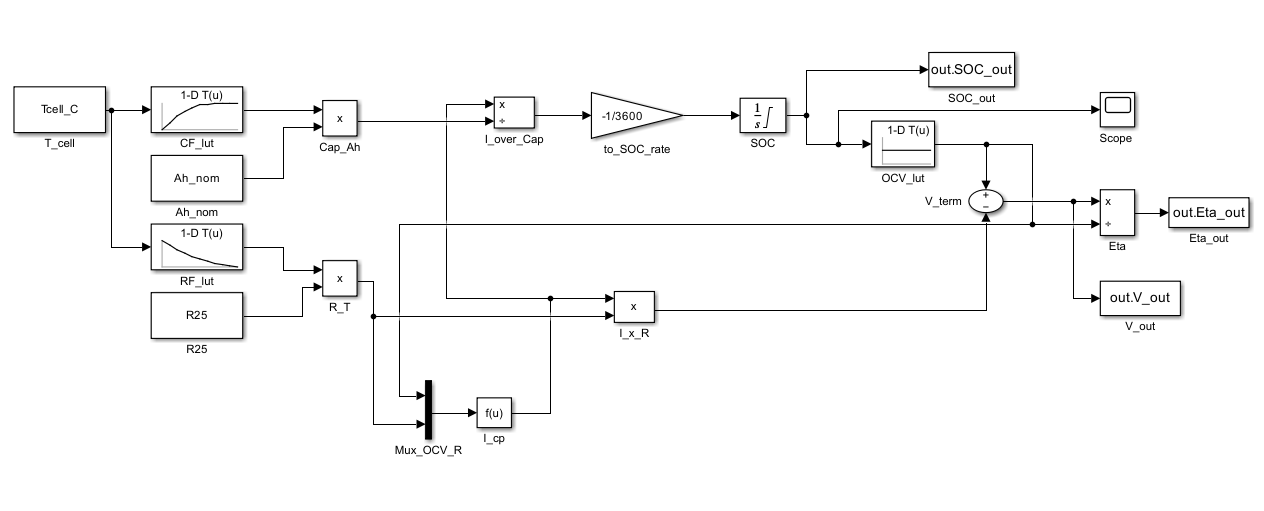
\includegraphics[width=\textwidth]{fig_simulink.png}
\caption{Block diagram of the Simulink model \texttt{easybike\_battery.slx}: temperature drives the capacity and resistance lookup tables; a function block solves the constant-power current; the integrator gives SOC.}
\label{fig:simulink}
\end{figure}

\subsection{Degradation, calibration and lifetime}
Cycle life falls with depth of discharge and temperature, and damage is accumulated month by month with Miner's rule \cite{miner1945}, as also done for variable-temperature VRLA service \cite{tsujikawa2009}:
\begin{align}
N_{eff,m}&=N_{80}\left(\frac{0.8}{\max(\mathrm{DoD}_m,0.05)}\right)^{k} f_T(T_m),\\
D&=n_{cyc}\sum_m \frac{w_m}{N_{eff,m}},\qquad L=\frac{1}{D\,d_{op}}\ \text{(years)},
\end{align}
where $w_m$ is the day-weighted share of month $m$, $d_{op}=300$ operating days per year and $n_{cyc}=1$. For LFP, $f_T=\min\{1,\exp[\tfrac{E_a}{R_g}(\tfrac1{T_K}-\tfrac1{298.15})]\}$ with $E_a=37.3$ kJ/mol \cite{yagci2026}; for lead-acid, $f_T=\min\{1,2^{-(T-25)/8}\}$ \cite{bu806a}. There is no life credit below 25\,$^\circ$C, and calendar ageing is not modelled.

The cycle life at 80\% DoD, $N_{80}$, is the least certain input: literature ranges (400 and 2{,}500 cycles) come from stationary storage. We therefore fit $N_{80}$ for each chemistry so that the modelled life at Khulna equals the survey median replacement interval. Because $N_{eff}$ is proportional to $N_{80}$ the fit is exact and unique. The fitted value is an \emph{effective field cycle life}: it also absorbs the unknown number of operating days, charging practice and battery quality. Calibration uses the Khulna temperature series only; the other two sites then follow from temperature alone. Before calibration the model is run with the literature values and compared with the survey (Section~\ref{sec:valid}); this comparison is the main validation.

\subsection{Total cost of ownership}
The 5- and 10-year net present cost with discount rate $r$ is
\begin{equation}
\mathrm{TCO}_H=C_0+\sum_{j=1}^{K}\frac{C_0(1-s)}{(1+r)^{jL}}-\frac{C_0\,\rho_H}{(1+r)^{H}}+\sum_{t=1}^{H}\frac{E_{grid}\,d_{op}\,\tau + m\,C_0}{(1+r)^t},
\end{equation}
with $C_0$ the set price, $K=\lfloor H/L\rfloor$ replacements, $s$ the resale fraction, $\rho_H$ the residual life fraction at horizon $H$, $\tau$ the tariff and $m$ the maintenance fraction. Cost per km is $\mathrm{TCO}_{10}$ divided by the discounted distance. Only battery-related cost is counted. Break-even set price and life are found by bisection on $\mathrm{TCO}_{10}(\mathrm{LFP})=\mathrm{TCO}_{10}(\mathrm{LA})$.

\subsection{Carbon, lead and policy}
Annual emissions per bike are $E_{CO_2}=E_{grid}\,d_{op}\,EF_{grid}+\varepsilon\,Q_{nom}\,12/L_{mo}$, with $EF_{grid}=0.62$ tCO$_2$/MWh \cite{doe_gef}, $Q_{nom}$ the pack energy, $L_{mo}$ the life in months and $\varepsilon=40$ and 50 kg CO$_2$e/kWh for LA and LFP \cite{jasper2025}. LFP packs are imported, so $\varepsilon$ is tested up to 110. Informal-smelting emissions have no verified factor and are excluded, which biases the lead-acid footprint downward. Lead cycled per year is $M_{Pb}=N\,m_{Pb}\,12/L_{mo}$ with $m_{Pb}$ = 56, 84 and 125 kg per lead-acid set: a mass flow, not an emission or a dose. Conversion scenarios move 0, 25, 50 and 100\% of a 1.4 M fleet from LA to LFP; outputs scale linearly. The \emph{operator support} needed is the 10-year cost gap per bike times the number converted, and the implied abatement cost is that gap divided by ten years of CO$_2$e saved. These quantities are indicative: they ignore health benefits, taxes and import costs.

\subsection{Validation and sensitivity}
Checks are: V1 data integrity (24 monthly values per site, none missing); V2 model life against survey replacement intervals, before and after calibration; V3 grid energy per bike-day against the 8--9 kWh per charge of the field study \cite{chowdhury2026} and the CLEAN and UNCTAD fleet figures \cite{clean2024,unctad_smep} (not used for calibration, so independent); V4 Simulink against the analytic model; V5 consistency of the survey's range complaints with ageing-limited life. One-at-a-time sensitivity over eleven inputs (\figref{tornado}) uses ranges taken from the survey wherever it supplies one.

\section{Results}
\label{sec:results}
\subsection{Survey results}
\label{sec:surveyres}
Of the \nSurvey{} respondents, \nLA{} (\shareLA\%) use lead-acid batteries, \nPW{} (\sharePW\%) reported a ``Powder'' battery of unconfirmed chemistry, and only \nLFP{} (\shareLFP\%) use LFP (\figref{survey1}, Table~\ref{tab:survey}). If Powder is a lead-based variant, lead-based batteries account for 38 of 43 drivers (88\%). The commonest set has four batteries (\fourBat{} of \nSurvey{} drivers), \onePerDay{} of \nSurvey{} charge once a day, and mean daily distance is \kmAll{} km (lead-acid \kmMeanLA{}, LFP \kmMeanLFP{}, Powder \kmMeanPW{} km; \figref{survey2}).
\begin{figure}[t]
\centering
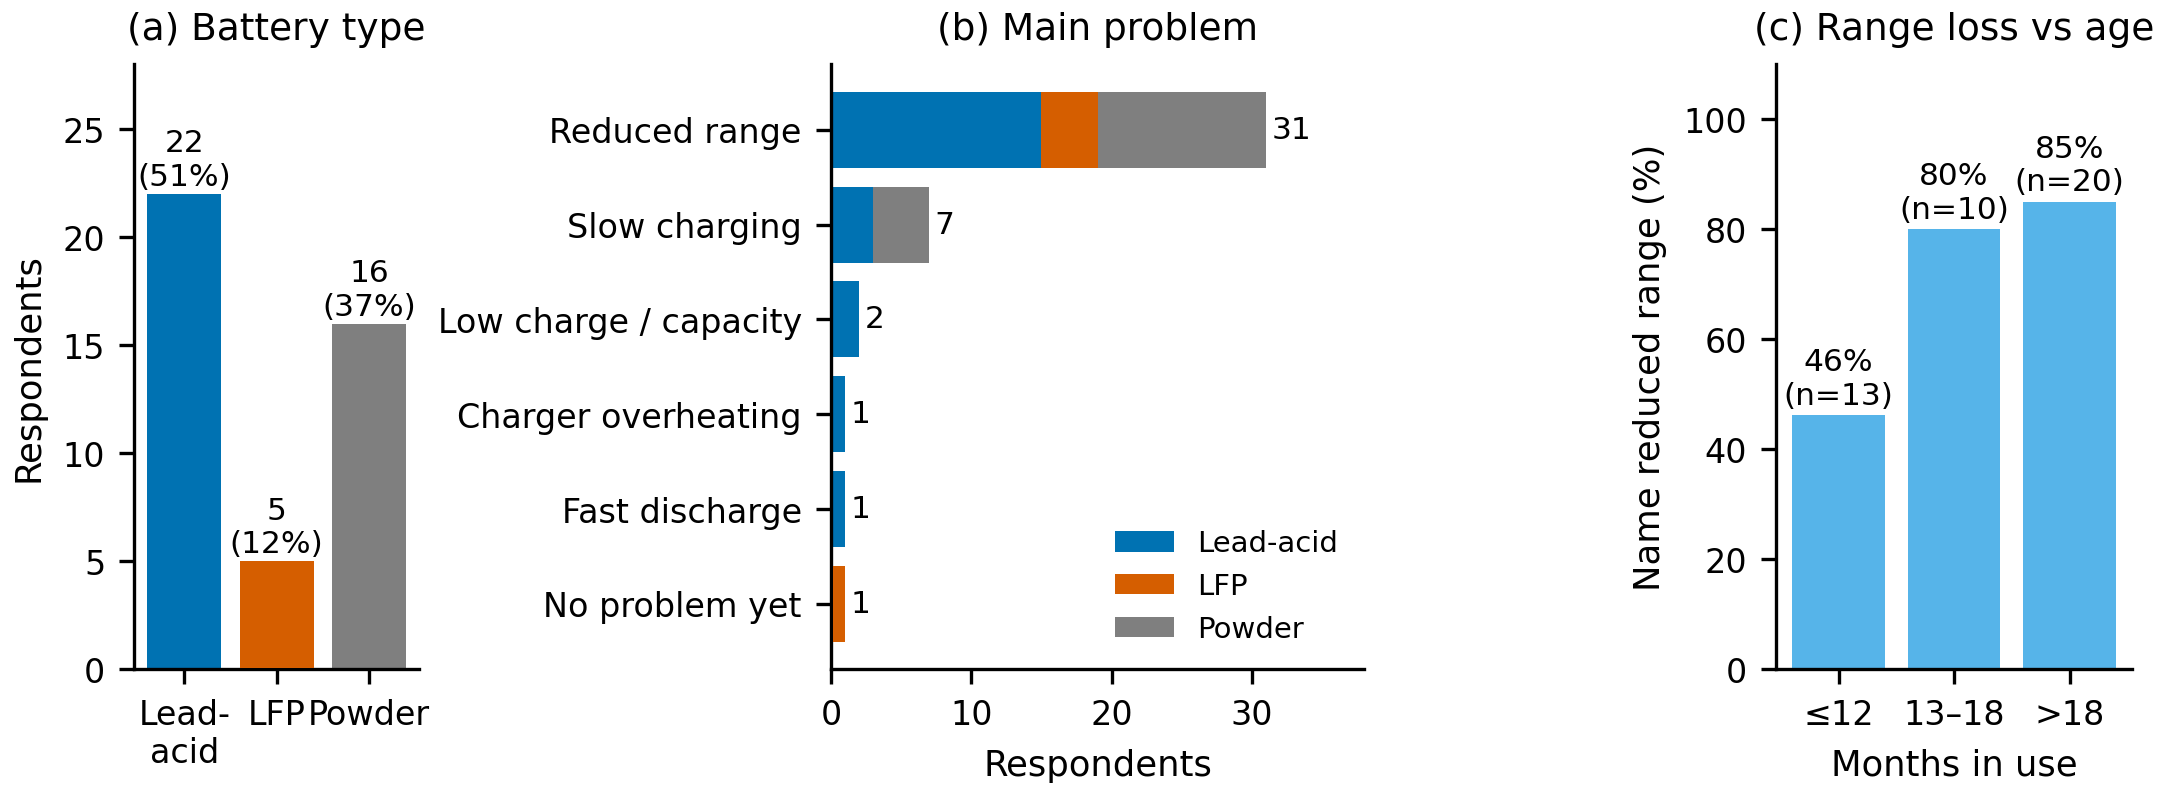
\includegraphics[width=\textwidth]{fig_survey_overview.png}
\caption{Survey sample ($n$ = 43): (a) battery type; (b) main problem reported by type; (c) share naming reduced range by months in use of the current set.}
\label{fig:survey1}
\end{figure}
\begin{table}[t]
\caption{Survey results by battery type ($n$ = 43 drivers, October 2026; source: author's field survey, cleaned data). Cost is the purchase price of the current set (BDT); replacement interval is the mid-point of the reported range (months; number of answers in brackets); resale is the mean of individual resale/purchase ratios.}
\label{tab:survey}
\centering\footnotesize
\resizebox{\textwidth}{!}{\begin{tabular}{lrrrrrrr}
\hline
Battery type & $n$ & Median cost & Mean cost & Daily km (mean) & Months in use (mean) & Median repl. interval & Resale / cost (\%) \\
\hline
Lead-acid & 22 & 29{,}000 & 46{,}318 & 83.0 & 14.1 & 18 (21) & 43 \\
Lithium (LFP) & 5 & 100{,}000 & 105{,}400 & 106.2 & 18.4 & 43.5 (4) & 13 \\
Powder & 16 & 28{,}000 & 32{,}906 & 56.9 & 21.0 & 30 (16) & 36 \\
All & 43 & 28{,}500 & 48{,}198 & 76.0 & 17.2 & 30 (41) & 37 \\
\hline
\end{tabular}}
\end{table}

The median purchase price of a lead-acid set is BDT \costMedLA{} against BDT \costMedLFP{} for LFP, a ratio of \costRatio. The lead-acid mean (BDT \costMeanLA{}) is much higher than the median because seven entries are BDT 60{,}000 or more, so medians are used. Drivers expect to replace a lead-acid set after a median \replMedLA{} months (mean \replMeanLA{}; range \replMinLA--\replMaxLA{}) and an LFP set after \replMedLFP{} months (range \replMinLFP--\replMaxLFP{}); Powder users report \replMedPW{} months. Resale value of the old set is \resaleRatioLA\% of purchase price for lead-acid and \resaleRatioLFP\% for LFP. Reduced range is the main problem for \rangeN{} of \nSurvey{} drivers (\rangeShare\%), and its share rises with the age of the set from \rngAgeA\% (up to 12 months) to \rngAgeB\% (13--18 months) and \rngAgeC\% (over 18 months; Table~\ref{tab:problems}).
\begin{figure}[t]
\centering
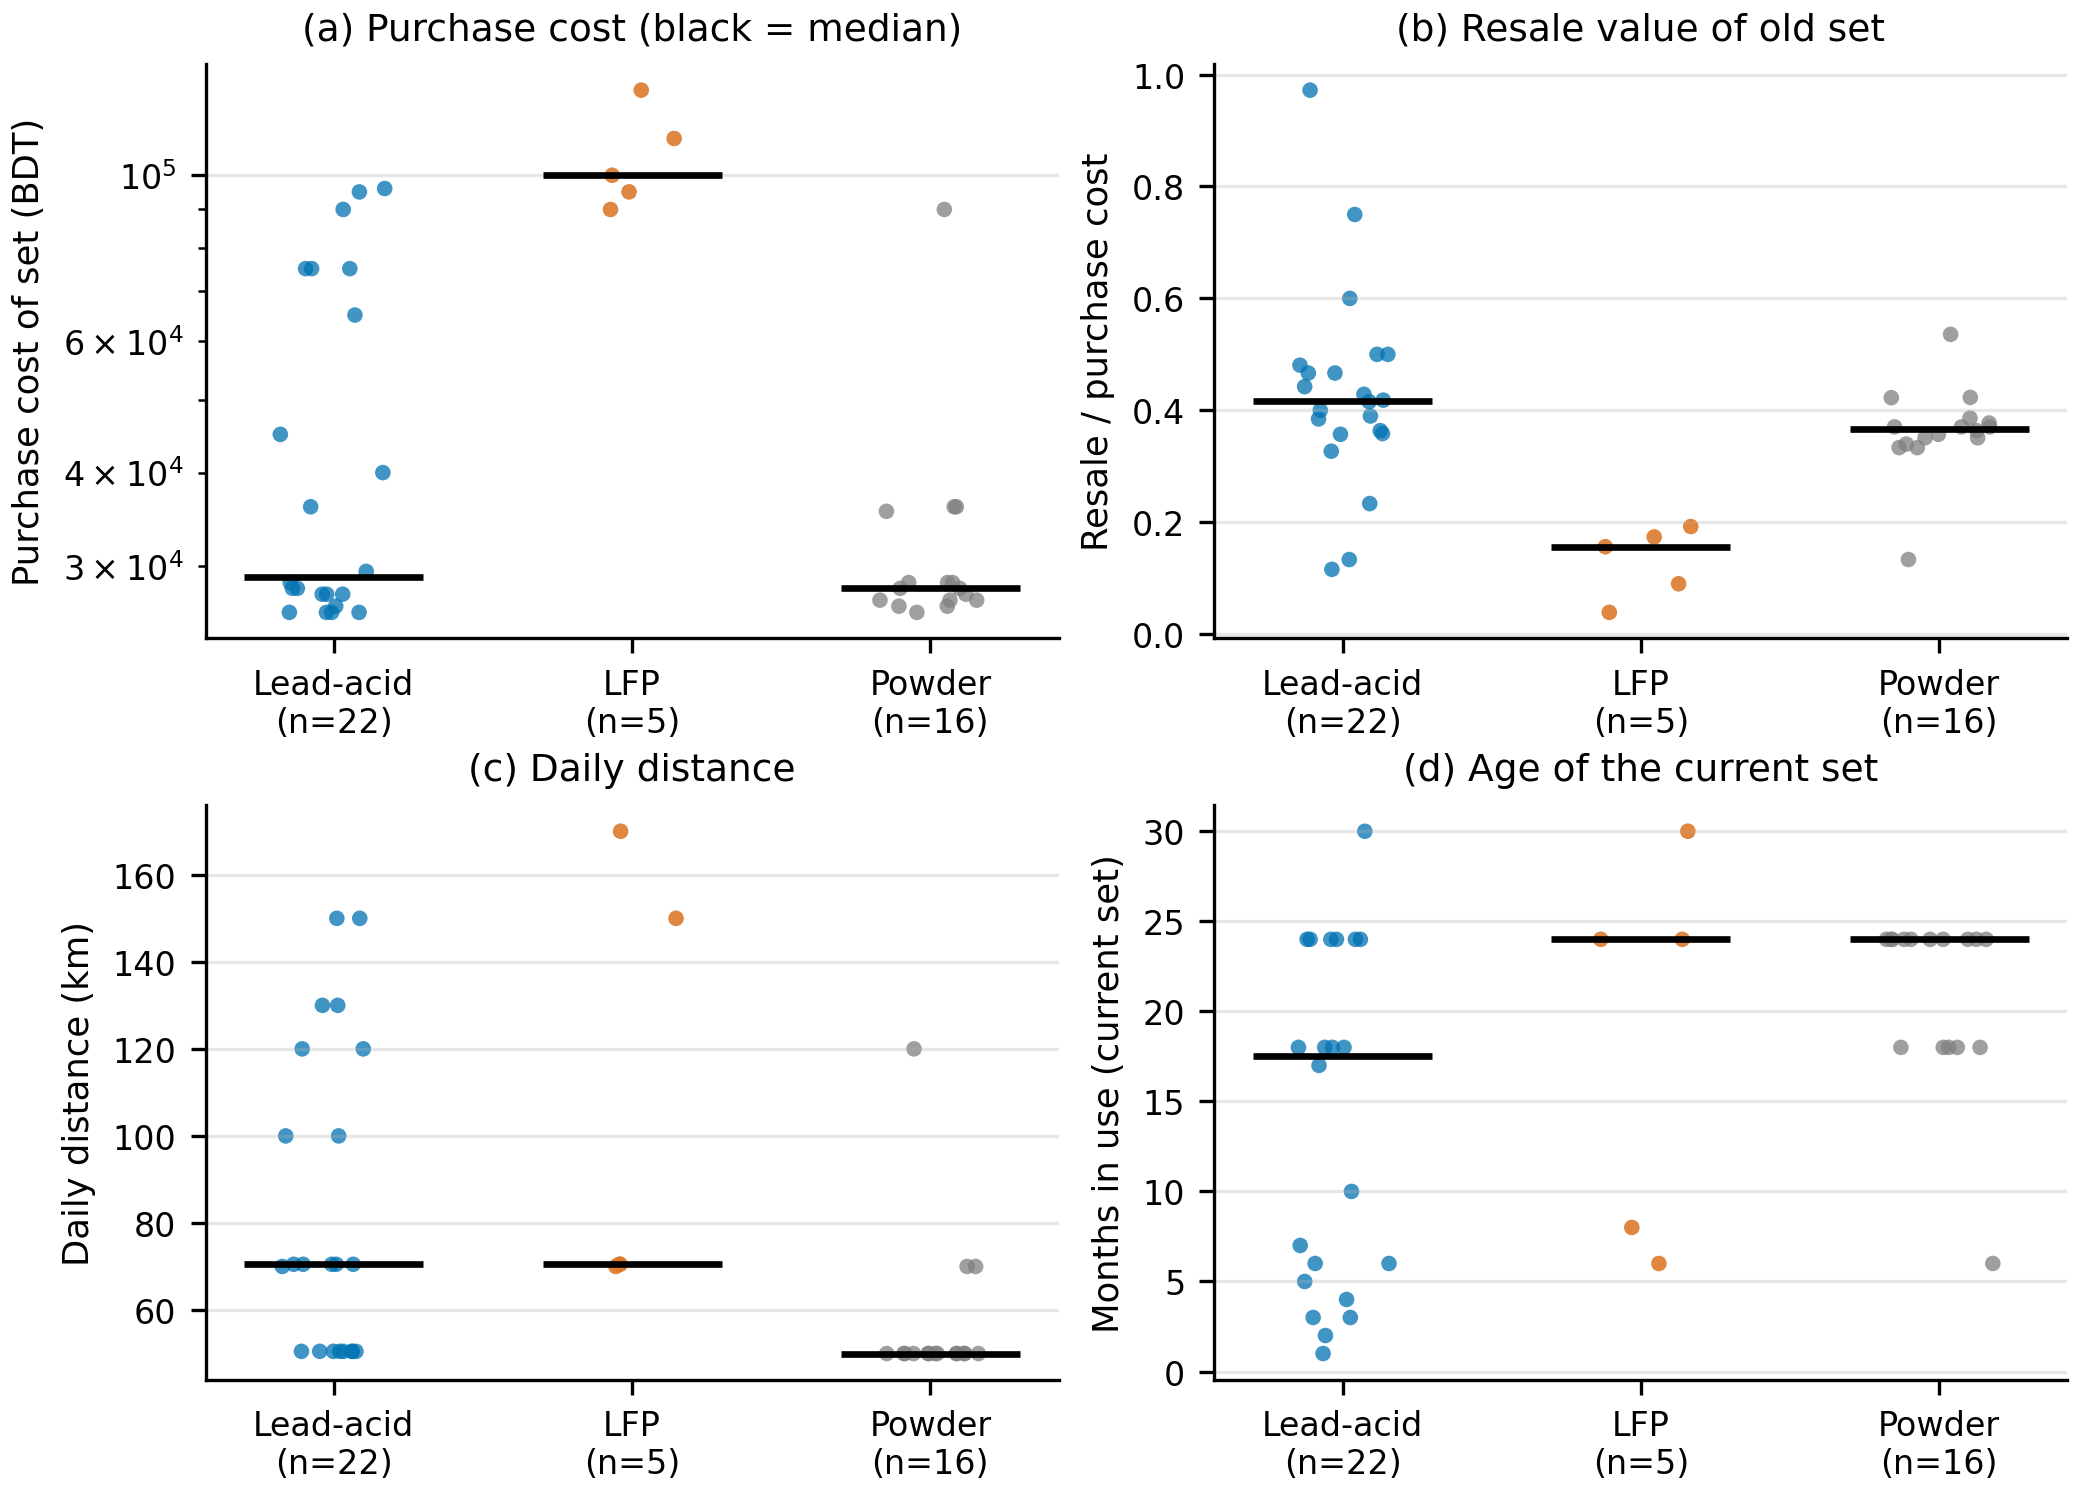
\includegraphics[width=0.9\textwidth]{fig_survey_cost_distance.png}
\caption{Survey answers by battery type (points; black bars = medians): (a) purchase cost of the current set (log scale); (b) resale/purchase ratio of the old set; (c) daily distance; (d) months in use.}
\label{fig:survey2}
\end{figure}
\begin{table}[t]
\caption{Main problem reported with the current battery (one answer per respondent) and, in the lower block, the share naming reduced range by battery-set age.}
\label{tab:problems}
\centering\footnotesize
\begin{tabular}{lrrrrr}
\hline
Problem & Lead-acid & LFP & Powder & All & Share (\%) \\
\hline
Reduced range & 15 & 4 & 12 & 31 & 72.1 \\
Slow charging & 3 & 0 & 4 & 7 & 16.3 \\
Low charge / capacity & 2 & 0 & 0 & 2 & 4.7 \\
Charger overheating & 1 & 0 & 0 & 1 & 2.3 \\
Fast discharge & 1 & 0 & 0 & 1 & 2.3 \\
No problem yet & 0 & 1 & 0 & 1 & 2.3 \\
\hline
\multicolumn{6}{l}{\emph{Reduced range by age of the current set}} \\
Up to 12 months ($n$=13) & \multicolumn{4}{r}{} & 46 \\
13--18 months ($n$=10) & \multicolumn{4}{r}{} & 80 \\
Over 18 months ($n$=20) & \multicolumn{4}{r}{} & 85 \\
\hline
\end{tabular}
\end{table}


\subsection{Calibration and validation}
\label{sec:valid}
\begin{table}[t]
\caption{Model checked against the survey and published figures (Khulna). Model (literature) uses the cycle lives of the data file (400 lead-acid, 2{,}500 LFP at 80\% DoD); model (calibrated) uses the survey-anchored values.}
\label{tab:valid}
\centering\footnotesize
\resizebox{\textwidth}{!}{\begin{tabular}{lrrrl}
\hline
Quantity & Survey / published & Model (literature) & Model (calibrated) & Outcome \\
\hline
Lead-acid replacement interval (months) & 18 (n=21; 95\% CI 17.5--30.0) & 7.8 & 18.0 & literature value 57\% below survey; calibrated \\
LFP replacement interval (months) & 43.5 (n=4; range 30--54) & 70.6 & 43.5 & literature value 62\% above survey; calibrated \\
Grid energy per bike-day, lead-acid (kWh) & 8--9 per charge (field study); 9.6 (CLEAN); 9.2 (UNCTAD) & -- & 8.4 & independent: 9--13\% below the published figures \\
Lead-acid set price (BDT) & 29{,}000 (median, n=22) & -- & 29{,}000 & input \\
LFP set price (BDT) & 100{,}000 (median, n=5) & -- & 100{,}000 & input \\
Charges per day & 1 (42 of 43 drivers) & -- & 1 & input \\
Reduced range as main problem & 72.1\% (rising with age) & -- & -- & consistent with ageing-limited life \\
\hline
\end{tabular}}
\end{table}

With the literature cycle lives (400 lead-acid, 2{,}500 LFP) the model gives a lead-acid life of \litLifeLA{} months at Khulna, \litErrLAabs\% below the survey median of \replMedLA{} months, and an LFP life of \litLifeLFP{} months, \litErrLFP\% above the survey median of \replMedLFP{} months (\figref{validlife}, Table~\ref{tab:valid}). The literature values therefore understate field life for lead-acid and overstate it for LFP. Fitting $N_{80}$ to the survey medians gives \NcalLA{} cycles for lead-acid and \NcalLFP{} for LFP. The survey interval for lead-acid has wide uncertainty (95\% bootstrap interval \ciLAlo--\ciLAhi{} months); if the ten lead-acid entries of 27 October (nine of them with the same 30-month interval) are excluded, the median is \replLAnobatch{} months ($n$ = \nLAnobatch{}). The LFP median rests on four answers (interval \ciLFPlo--\ciLFPhi{} months), and these are expectations because the sets are on average only \ageMeanLFP{} months old.
\begin{figure}[t]
\centering
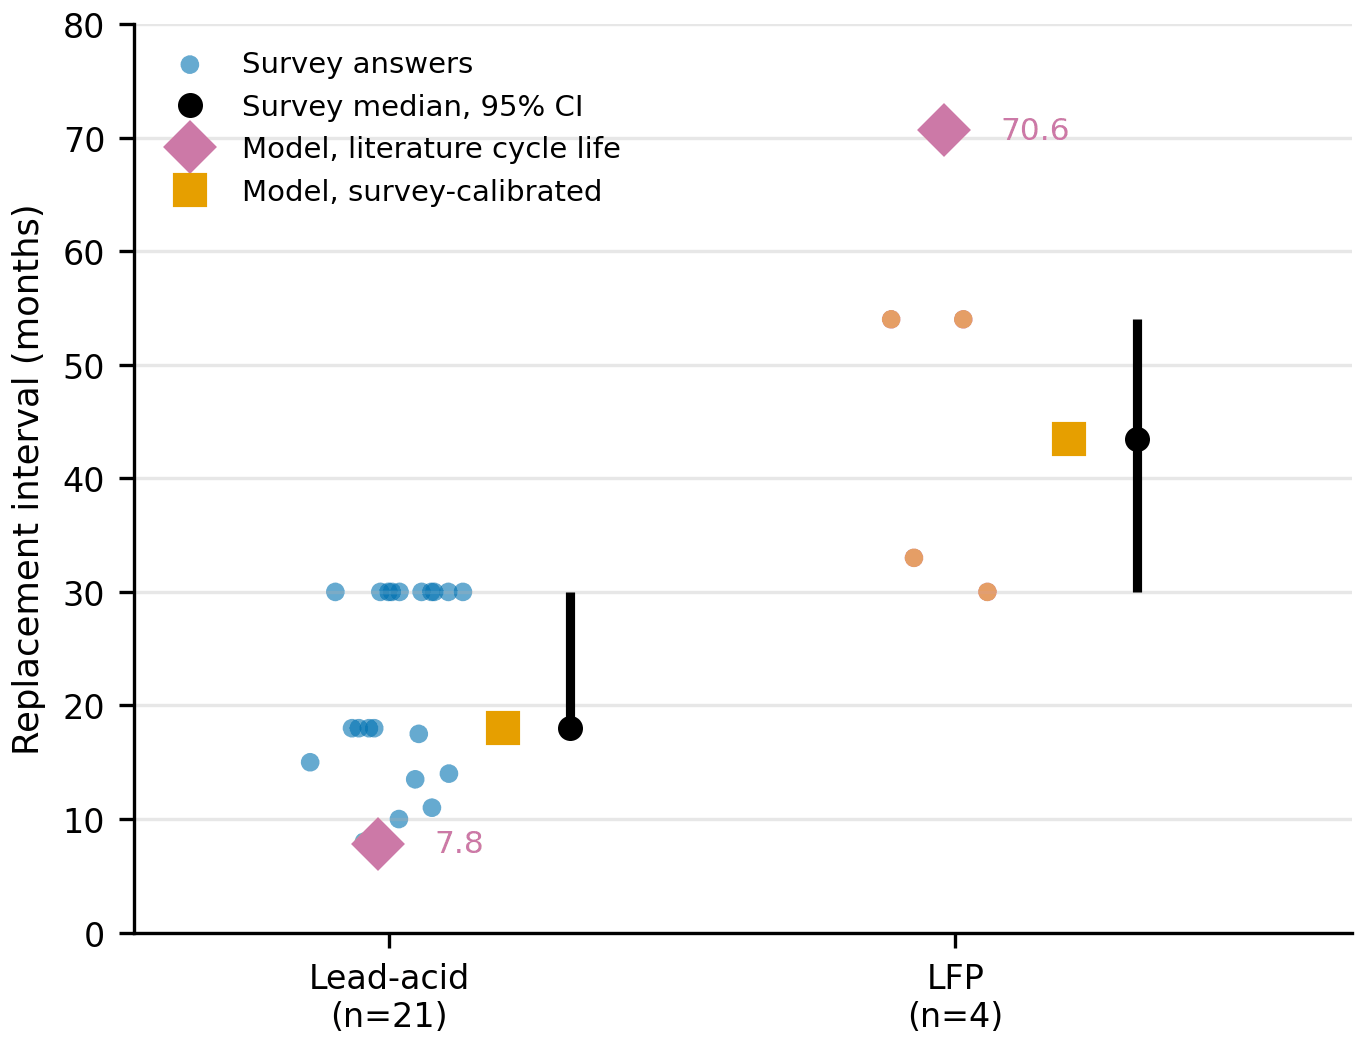
\includegraphics[width=0.6\textwidth]{fig_valid_life.png}
\caption{Validation of battery life at Khulna: survey replacement intervals (points), survey median with 95\% bootstrap interval, the model with literature cycle lives (diamond) and the survey-calibrated model (square).}
\label{fig:validlife}
\end{figure}
Three checks are independent of the calibration. Modelled lead-acid grid energy is \vEgrid{} kWh per bike-day, inside the 8--9 kWh per charge reported by the field study \cite{chowdhury2026} and \vCleanPct\% below the \vClean{} kWh implied by the CLEAN totals \cite{clean2024} and \vUnctadPct\% below the \vUnctad{} kWh per vehicle-day implied by 4{,}600 MWh/day for an estimated 500{,}000 autorickshaws, a figure reported by UNCTAD from Al-Amin and Sahabuddin \cite{unctad_smep,alamin2023} (the same brief's highlight box attributes it to 4 M vehicles, which is inconsistent and is not used). The Simulink and analytic models agreed in all twelve cases of the verification run (Appendix~\ref{app:sim}). Finally, the rise in range complaints with age (\figref{survey1}c) is consistent with ageing-limited life. The model is therefore checked against survey and published ranges, but it is not validated against metered operating data.

\subsection{Temperature and battery performance}
Monthly mean T2M follows the same seasonal cycle at all three sites, from about \Tmin\,$^\circ$C in January to \Tmax\,$^\circ$C in April 2024 (\figref{temp}). Mean battery temperature is \TcKhulna, \TcChuadanga\ and \TcRajshahi\,$^\circ$C, a spread of \Tspread\,$^\circ$C. Because the calibration is made at Khulna, modelled life differs between sites only through temperature: \lifeLAKhulna, \lifeLAChuadanga\ and \lifeLARajshahi{} months for lead-acid and \lifeLFPKhulna, \lifeLFPChuadanga\ and \lifeLFPRajshahi{} months for LFP (Table~\ref{tab:results}).
\begin{figure}[t]
\centering
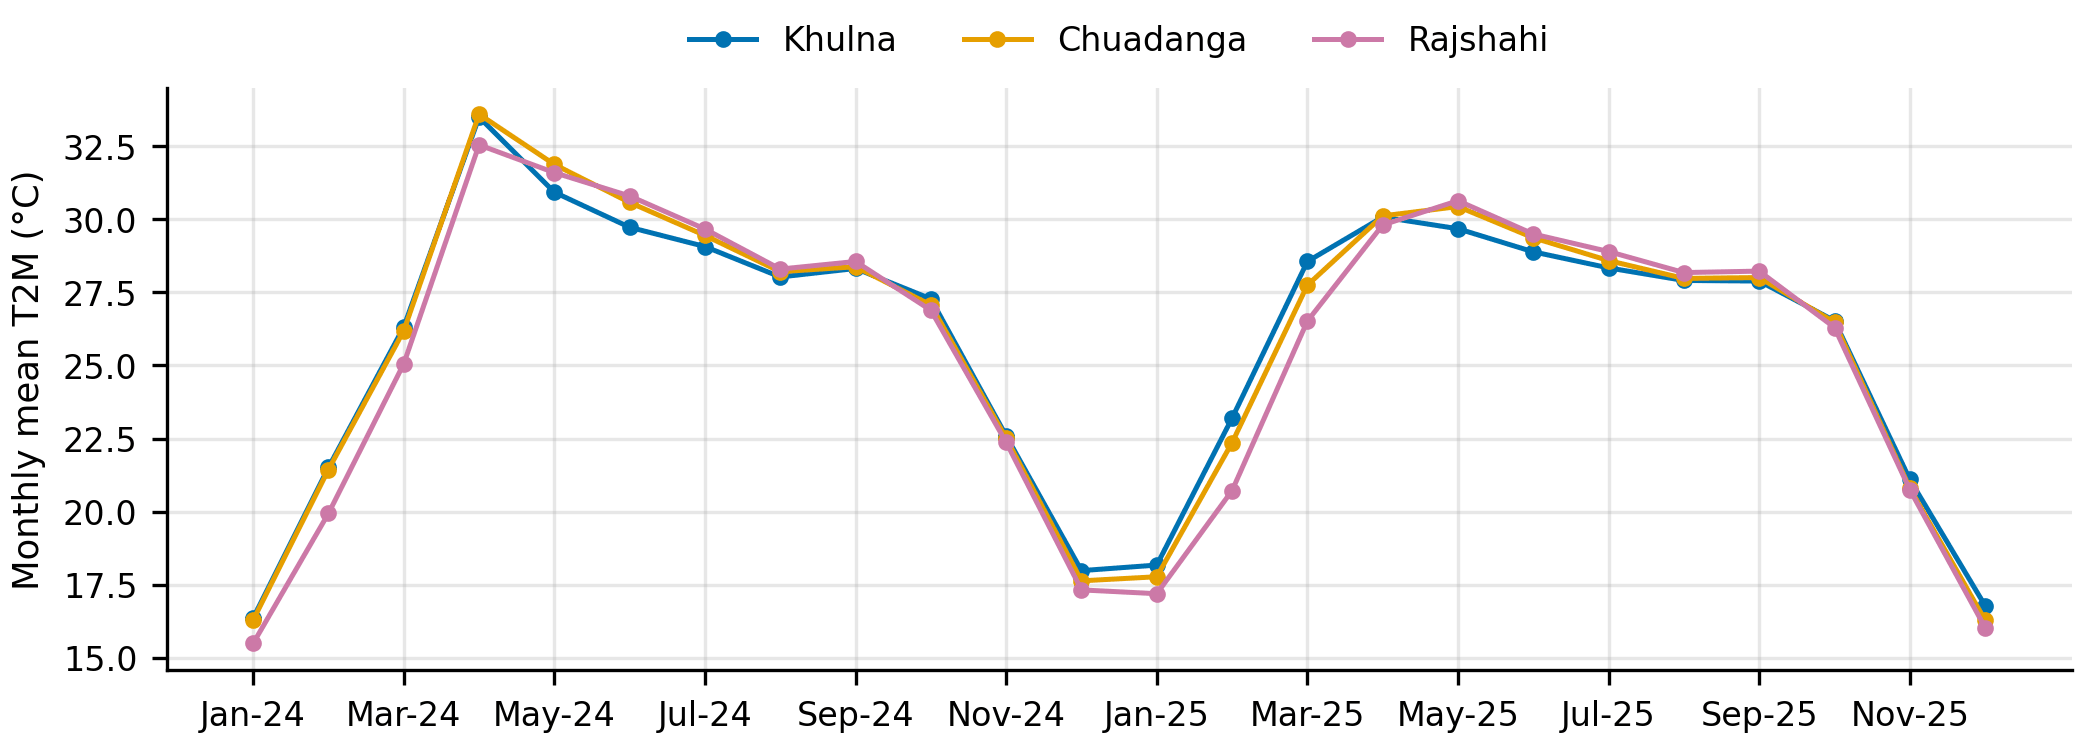
\includegraphics[width=0.9\textwidth]{fig1_temperature.png}
\caption{NASA POWER monthly mean 2\,m temperature at the three sites, Jan 2024--Dec 2025.}
\label{fig:temp}
\end{figure}
\begin{table}[t]
\caption{Survey-anchored model results for three sites (NASA POWER monthly $T_{2m}$, Jan 2024--Dec 2025; battery temperature = ambient + 5\,$^\circ$C). Cycle life is calibrated at Khulna so that modelled life equals the survey median replacement interval (18 months lead-acid, 43.5 months LFP); other sites differ only through temperature. TCO is net present cost at 11.96\% discount rate and BDT 11.36/kWh. Source: \texttt{results\_summary.csv} from \texttt{easybike\_main.m}.}
\label{tab:results}
\centering\footnotesize
\resizebox{\textwidth}{!}{\begin{tabular}{llrrrrrrrrr}
\hline
Site & Battery & $\bar T_{cell}$ & $\eta$ & DoD & Range & $E_{grid}$ & Life & Repl. & TCO$_{10}$ & Cost \\
 & & ($^\circ$C) & (\%) & (\%) & (km) & (kWh/d) & (mo) & (10 yr) & ($10^3$ BDT) & (BDT/km) \\
\hline
Khulna & Lead-Acid & 30.8 & 90.2 & 88.1 & 69.1 & 8.35 & 18.0 & 6 & 245 & 1.90 \\
 & LFP & 30.8 & 97.8 & 82.1 & 74.1 & 7.09 & 43.5 & 2 & 322 & 2.50 \\
\hline
Chuadanga & Lead-Acid & 30.8 & 90.2 & 88.1 & 69.1 & 8.36 & 17.8 & 6 & 247 & 1.91 \\
 & LFP & 30.8 & 97.8 & 82.1 & 74.0 & 7.09 & 43.3 & 2 & 323 & 2.50 \\
\hline
Rajshahi & Lead-Acid & 30.5 & 90.0 & 88.4 & 68.9 & 8.38 & 18.1 & 6 & 246 & 1.90 \\
 & LFP & 30.5 & 97.8 & 82.2 & 74.0 & 7.09 & 43.7 & 2 & 322 & 2.49 \\
\hline
\end{tabular}}
\end{table}

Discharge efficiency is \effLA\% for lead-acid and \effLFP\% for LFP, so LFP draws \gridratio\% less grid energy (\egLA{} versus \egLFP{} kWh per day). At \kmUsed{} km per day the lead-acid set runs at \dodLA\% mean depth of discharge (maximum \dodmaxLA\%), above the 80\% limit on which cycle life is rated, which is consistent with its short life; the LFP set runs at \dodLFP\% (maximum \dodmaxLFP\%). The modelled range to 80\% DoD is \rngLA{} km for lead-acid and \rngLFP{} km for LFP.
\begin{figure}[t]
\centering
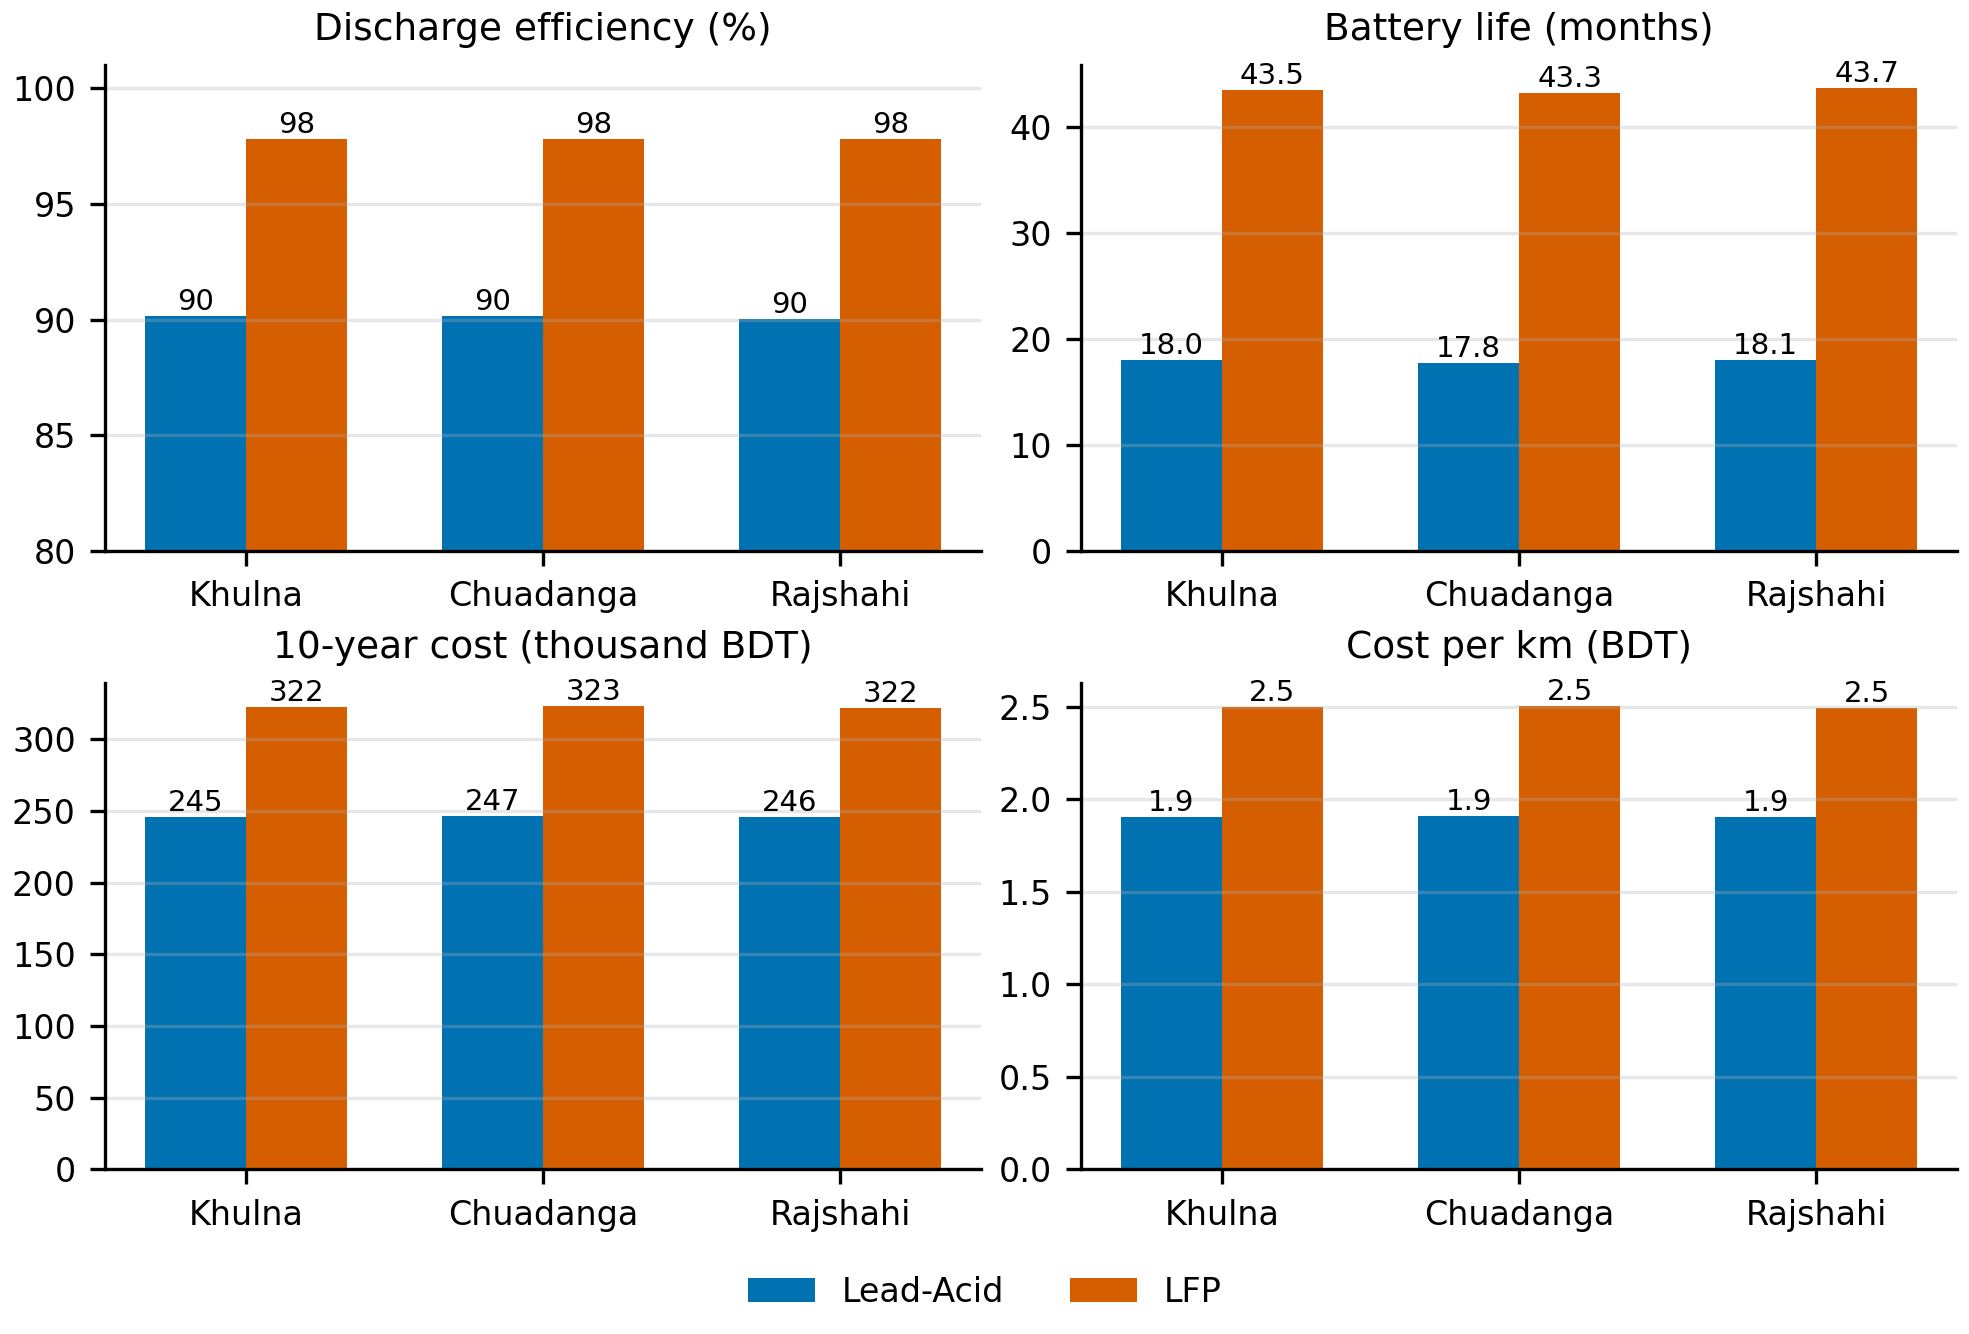
\includegraphics[width=0.85\textwidth]{fig2_comparison.png}
\caption{Site comparison of discharge efficiency, battery life, 10-year NPV cost and cost per km.}
\label{fig:comp}
\end{figure}
\begin{figure}[t]
\centering
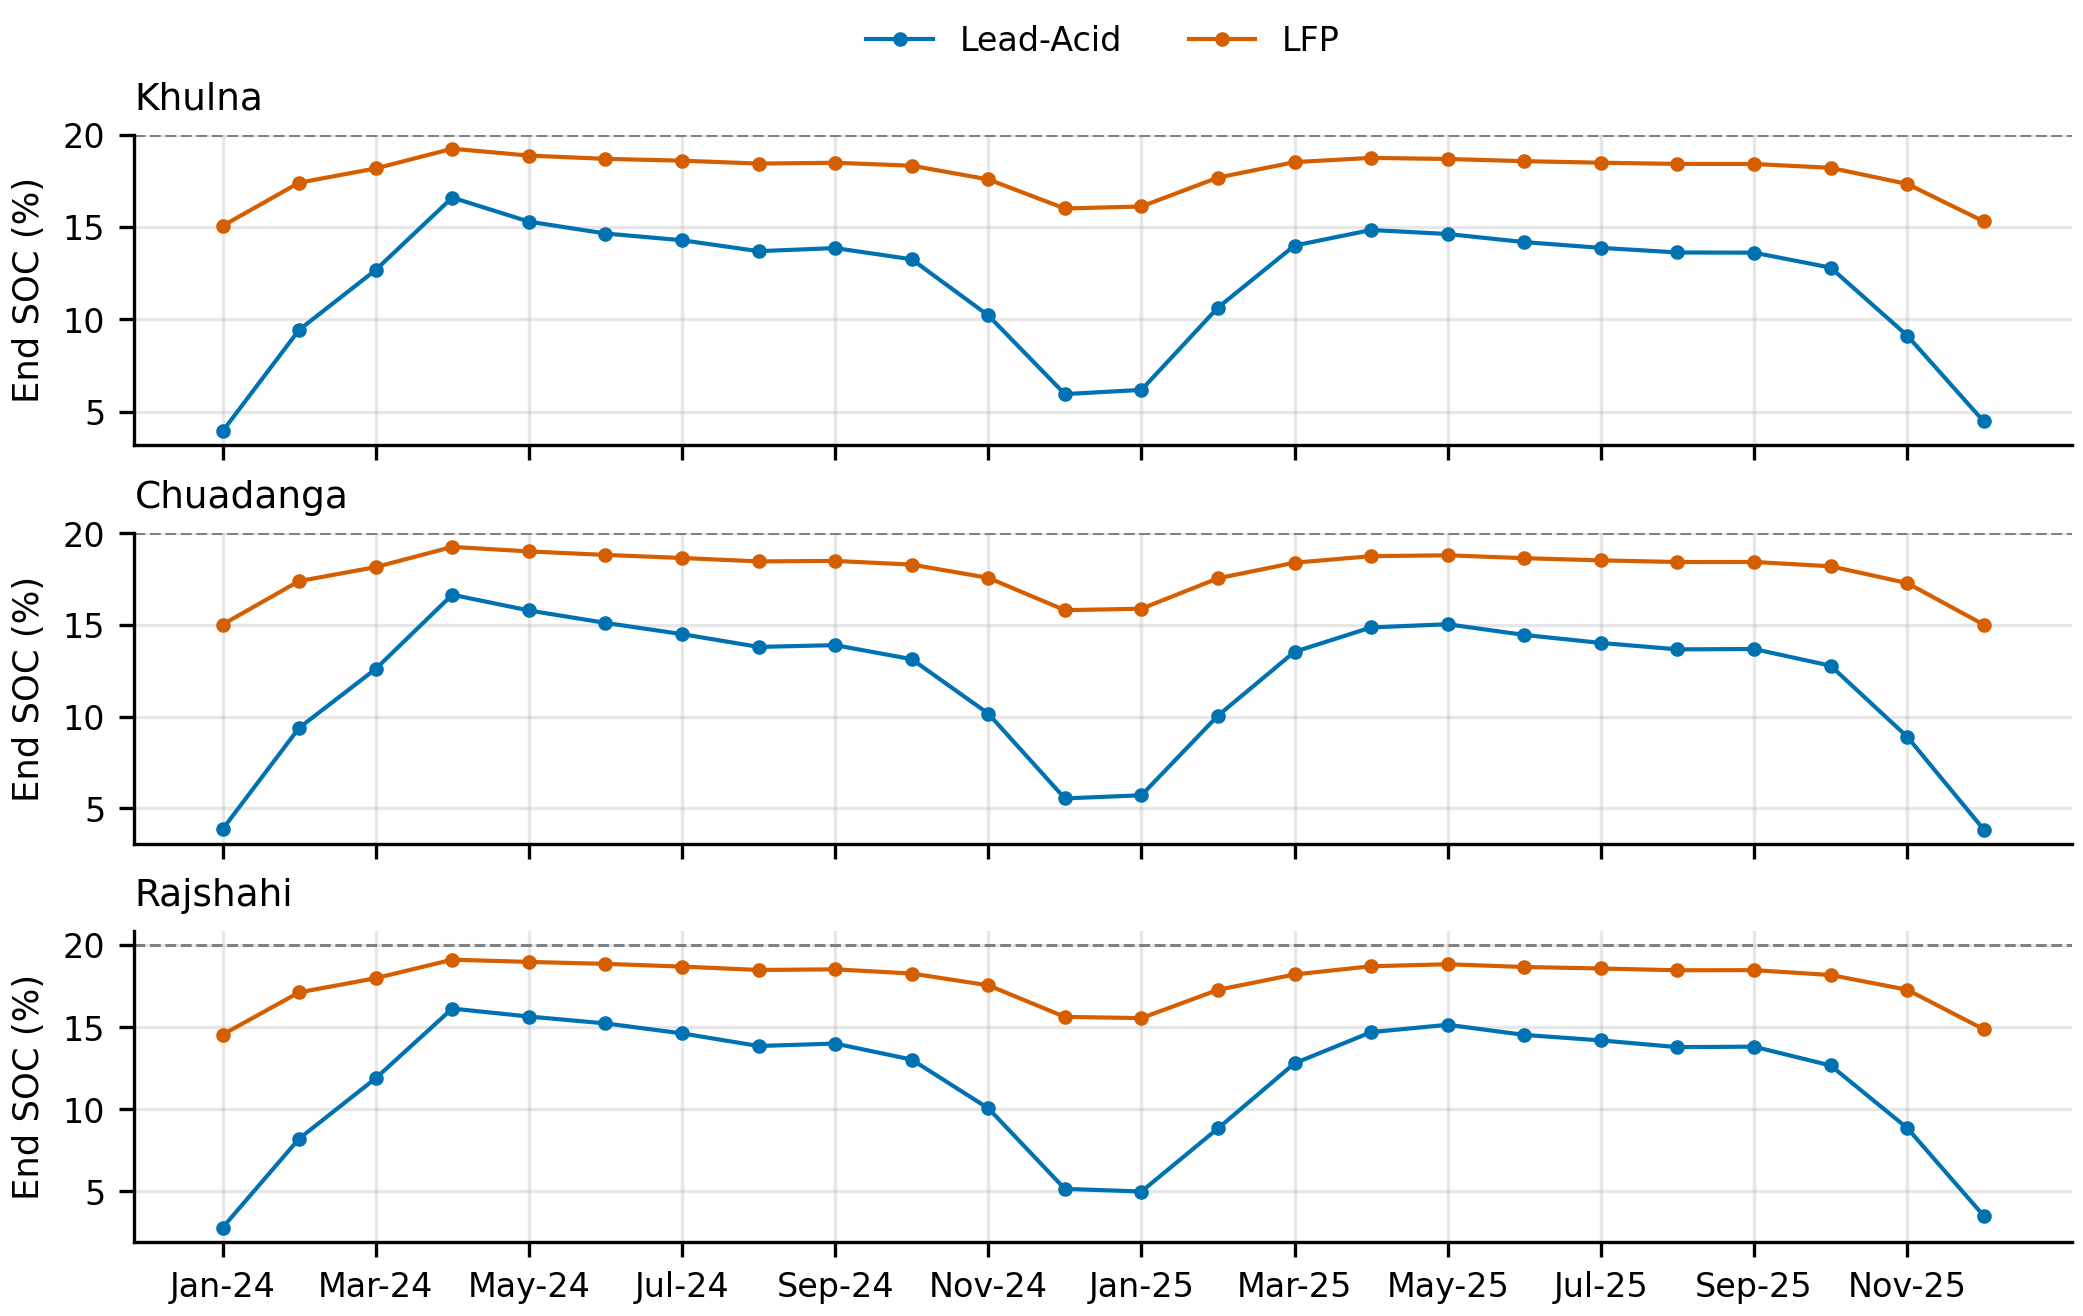
\includegraphics[width=0.85\textwidth]{fig3_soc.png}
\caption{Month-end state of charge after one day's discharge; dashed line = 20\% limit.}
\label{fig:soc}
\end{figure}

\subsection{Cost of ownership}
With survey-anchored inputs the ten-year net present cost per bike is BDT \tcoLA{} for lead-acid and BDT \tcoLFP{} for LFP (site mean): LFP costs BDT \gapLFP{} (\gapPct\%) \emph{more}, and its cost per km is BDT \cpkLFP{} against BDT \cpkLA{}. A lead-acid bike needs \repLA{} replacement sets in ten years and an LFP bike \repLFP{}, but each LFP set costs \costRatio{} times as much and is resold for a smaller share of its price (\figref{tco}). With the literature cycle lives the sign reverses: LFP would be BDT \litGap{} cheaper. Using drivers' own prices and intervals therefore changes the operator's conclusion.
\begin{figure}[t]
\centering
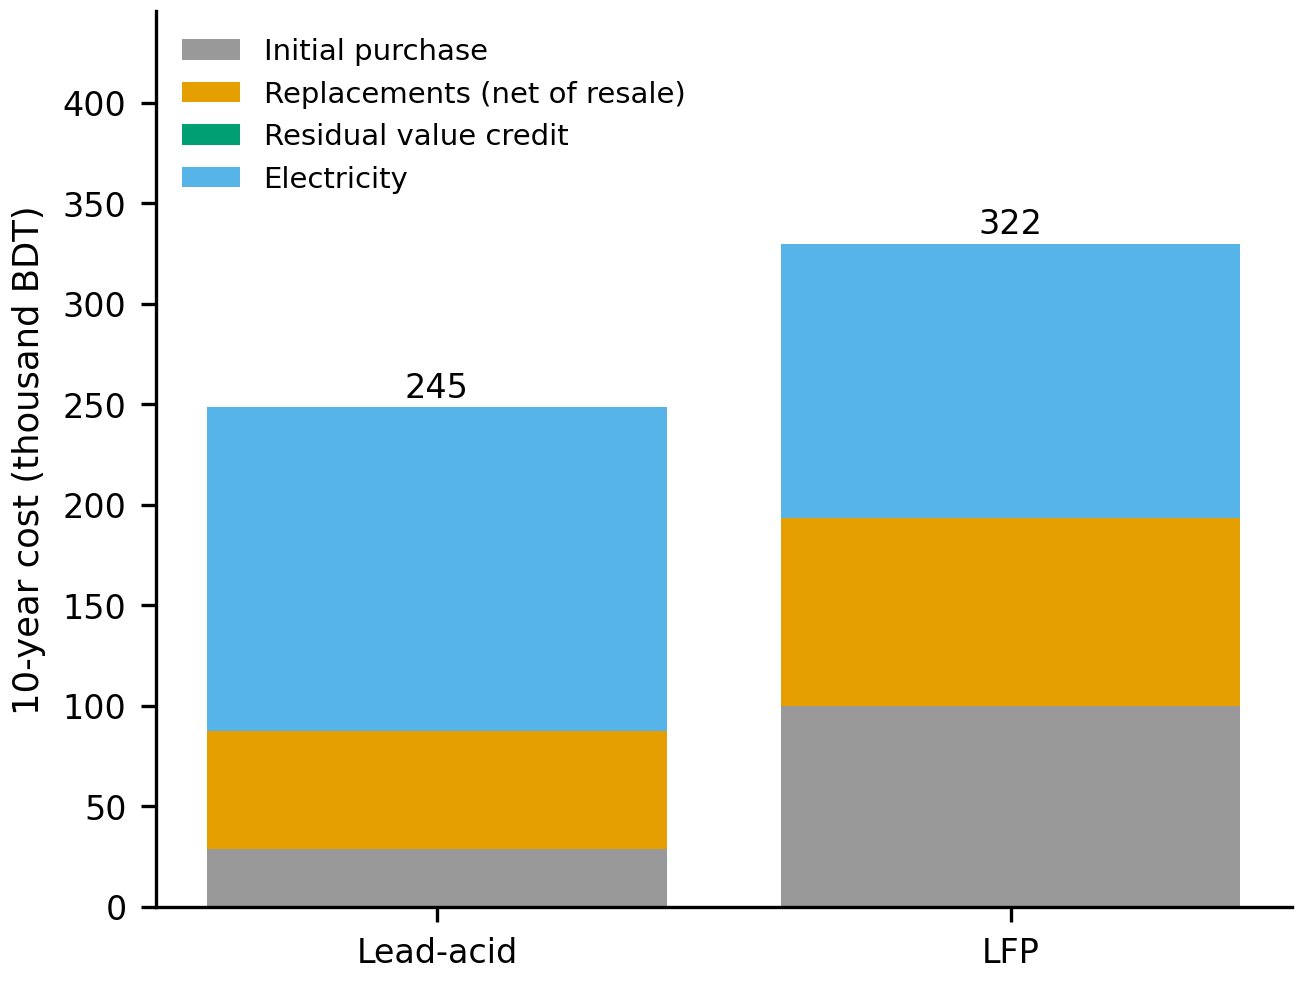
\includegraphics[width=0.55\textwidth]{fig_tco_breakdown.png}
\caption{Composition of the 10-year cost at Khulna (thousand BDT).}
\label{fig:tco}
\end{figure}

\subsection{Break-even, scenarios and sensitivity}
\label{sec:sens}
LFP matches lead-acid at a set price of BDT \beP{} (\bePpct\% below the survey median) if its life is \replMedLFP{} months, or at a life of \beL{} months if the price is BDT \priceLFP{} (\figref{breakeven}). The break-even price is BDT \bePA{} for a 30-month life, \bePB{} for 54 months, \bePC{} for 72 months and \bePD{} for 96 months. All five surveyed LFP set prices lie above the break-even line.
\begin{figure}[t]
\centering
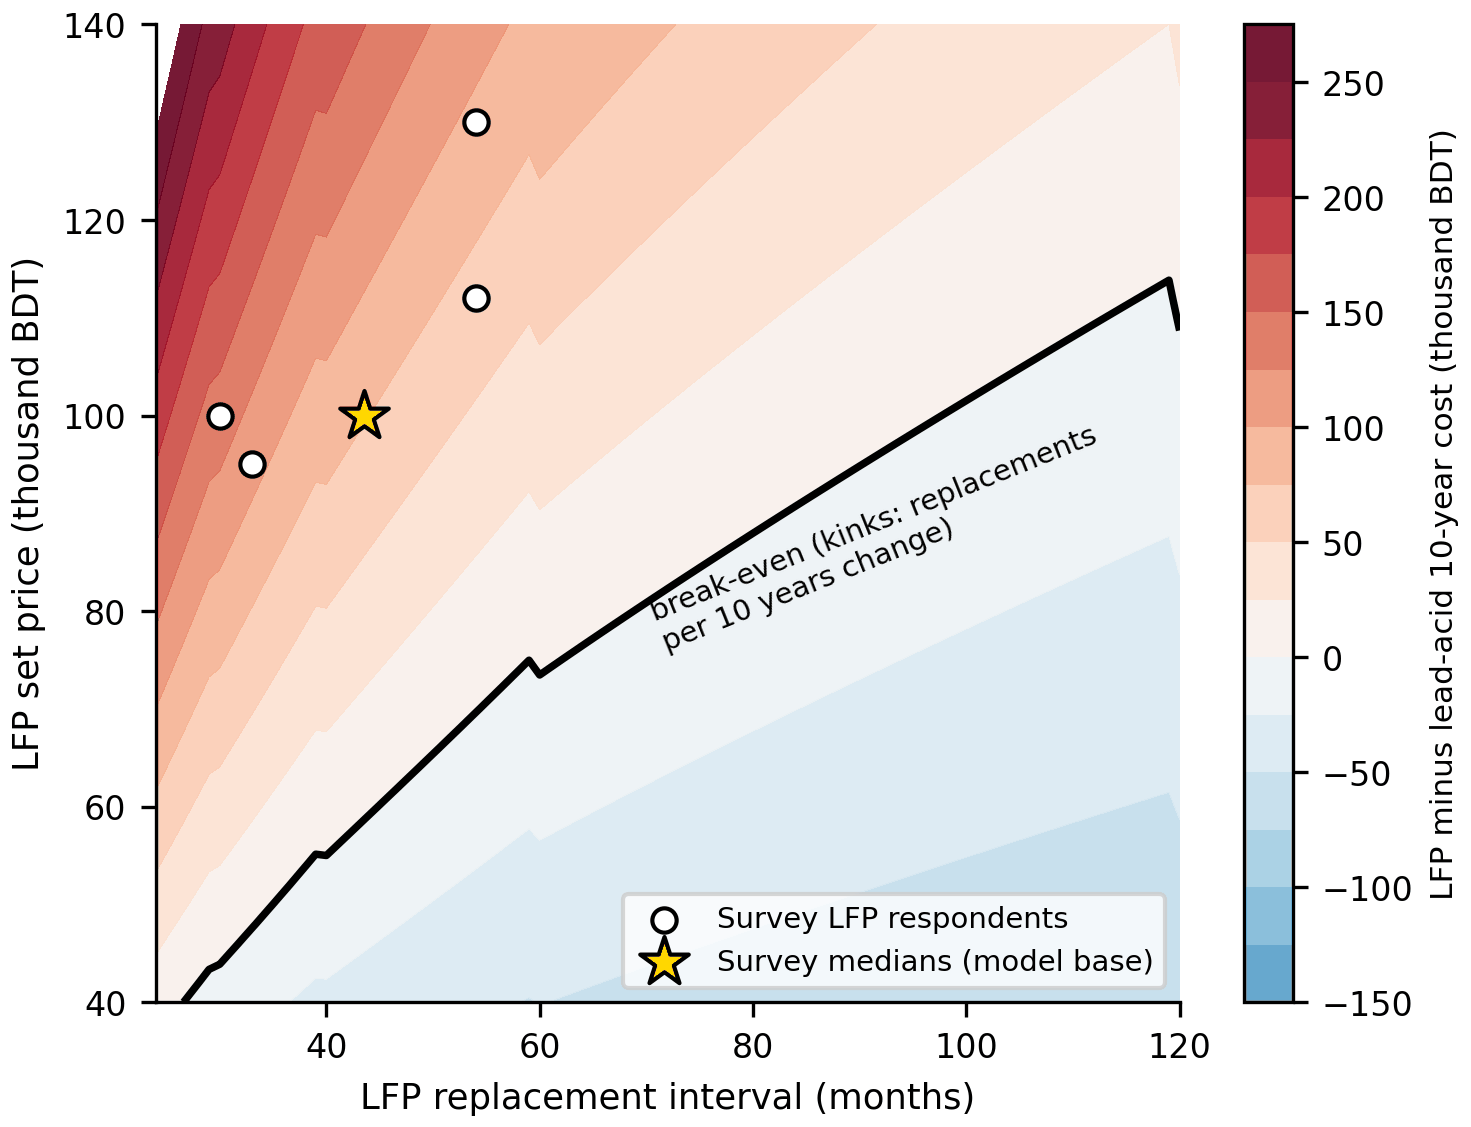
\includegraphics[width=0.62\textwidth]{fig_breakeven.png}
\caption{Ten-year cost of LFP minus lead-acid at Khulna as a function of LFP set price and replacement interval. Red: LFP dearer; blue: LFP cheaper. White circles: surveyed LFP drivers; star: survey medians. Kinks occur where the number of replacements in ten years changes.}
\label{fig:breakeven}
\end{figure}
\begin{table}[t]
\caption{Scenario runs. Upper block: battery temperature rise above ambient (site mean). Lower block: daily distance at Khulna (max DoD $>$100\% means the pack cannot serve the duty). Life in months; TCO in $10^3$ BDT.}
\label{tab:scen}
\centering\footnotesize
\resizebox{\textwidth}{!}{\begin{tabular}{lrrrrrr}
\hline
 & \multicolumn{2}{c}{Life (months)} & \multicolumn{2}{c}{10-yr TCO ($10^3$ BDT)} & \multicolumn{2}{c}{Max DoD (\%)} \\
Scenario & LA & LFP & LA & LFP & LA & LFP \\
\hline
$\Delta T$ = +0\,$^\circ$C & 23.8 & 51.6 & 236 & 300 & -- & -- \\
$\Delta T$ = +5\,$^\circ$C & 18.0 & 43.5 & 246 & 322 & -- & -- \\
$\Delta T$ = +10\,$^\circ$C & 12.5 & 35.3 & 269 & 352 & -- & -- \\
\hline
50 km/day & 32.3 & 66.1 & 161 & 229 & 63 & 56 \\
76 km/day & 18.0 & 43.5 & 245 & 322 & 96 & 85 \\
100 km/day & 12.3 & 33.1 & 328 & 408 & 126 & 112 \\
\hline
\end{tabular}}
\end{table}

Table~\ref{tab:scen} shows that battery temperature rise and daily distance change life and cost for both chemistries without changing the ranking. The tornado chart (\figref{tornado}) shows that the lead-acid life and LFP life and price dominate, and that the tariff, discount rate and operating days matter little. If lead-acid sets lasted only 8 months (the shortest survey answer) LFP would roughly break even (gap BDT \laEightGap{}); if they lasted 30 months (the longest) LFP would be BDT \laThirtyGap{} dearer. Combining the most favourable survey values for LFP (lead-acid life 8 months and price BDT 45{,}000, LFP life 54 months and price BDT 90{,}000) makes LFP BDT 147{,}457 cheaper; the most unfavourable combination makes it BDT \extUnfav{} dearer. Tariffs of BDT 7.70 and 16.24 per kWh leave the gap at BDT \tarLow{} and \tarHigh{}. A hot day at 42\,$^\circ$C ambient ages lead-acid \heatLA{} times and LFP \heatLFP{} times faster than the 2024--25 monthly-mean climate.
\begin{figure}[t]
\centering
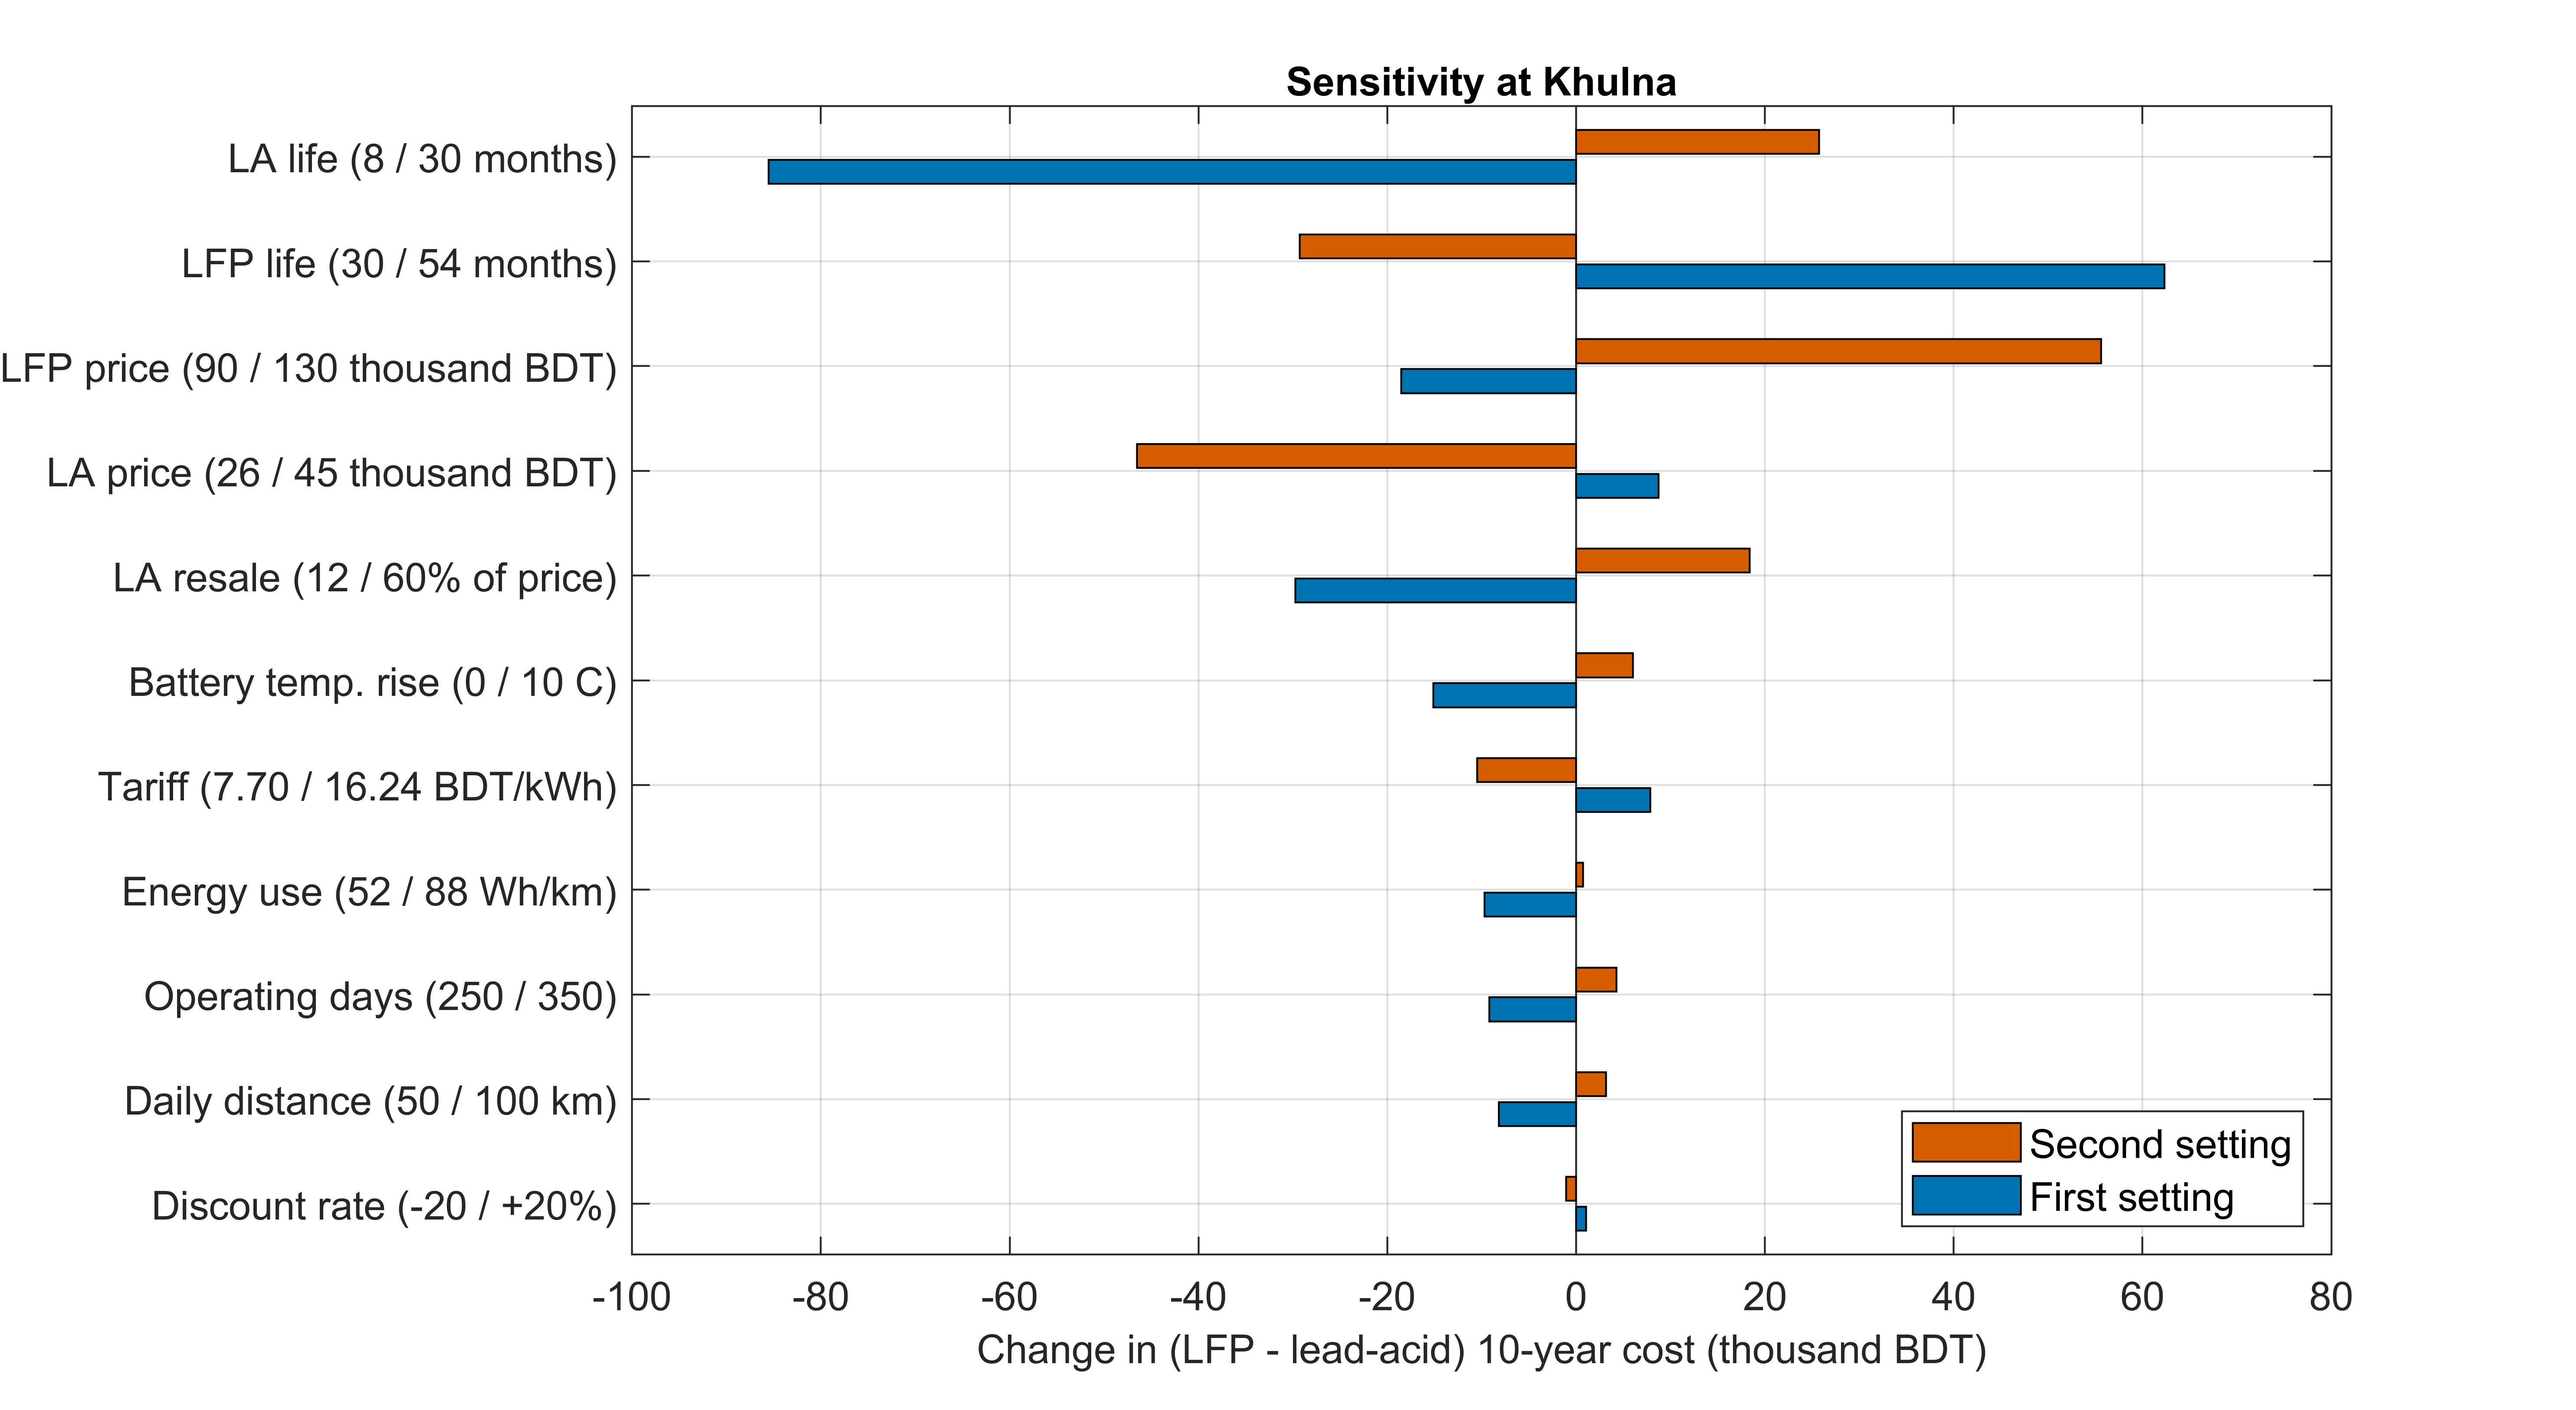
\includegraphics[width=0.9\textwidth]{fig4_tornado.png}
\caption{One-at-a-time sensitivity of the LFP-minus-LA 10-year cost gap at Khulna (base gap +\gapLFP{} BDT). Negative values favour LFP.}
\label{fig:tornado}
\end{figure}

\subsection{Carbon footprint, lead flow and policy scenarios}
A lead-acid easy-bike causes about \perbikeLA{} kg CO$_2$e per year and an LFP bike \perbikeLFP{} (Table~\ref{tab:co2bike}, \figref{co2}). Switching one bike saves \saveBike{} kg CO$_2$e per year, \saveOp{} from lower electricity use and \saveEmb{} from fewer manufactured sets (\packsLA{} lead-acid against \packsLFP{} LFP sets per year). For 1.4 M bikes this is \fleetA{} Mt CO$_2$e per year, or \fleetB{} Mt for 3 M bikes. The per-bike saving stays between \sensMin{} and \sensMax{} kg per year for LFP manufacturing footprints of 50--110 kg CO$_2$e/kWh and grid factors of 0.55--0.70 (\figref{co2sens}).
\begin{table}[t]
\caption{Carbon budget per bike per year (Khulna, survey-anchored lives; grid factor 0.62 tCO$_2$/MWh; manufacture and end-of-life 40 and 50 kg CO$_2$e per kWh of pack capacity for LA and LFP; pack energy 6.7 kWh for both).}
\label{tab:co2bike}
\centering\footnotesize
\begin{tabular}{lrrrr}
\hline
Battery & Packs/yr & Operation & Manuf.+EOL & Total \\
 & & (kg CO$_2$e) & (kg CO$_2$e) & (kg CO$_2$e) \\
\hline
Lead-acid & 0.67 & 1556 & 180 & 1736 \\
LFP & 0.28 & 1319 & 93 & 1412 \\
\hline
\end{tabular}
\end{table}

\begin{figure}[t]
\centering
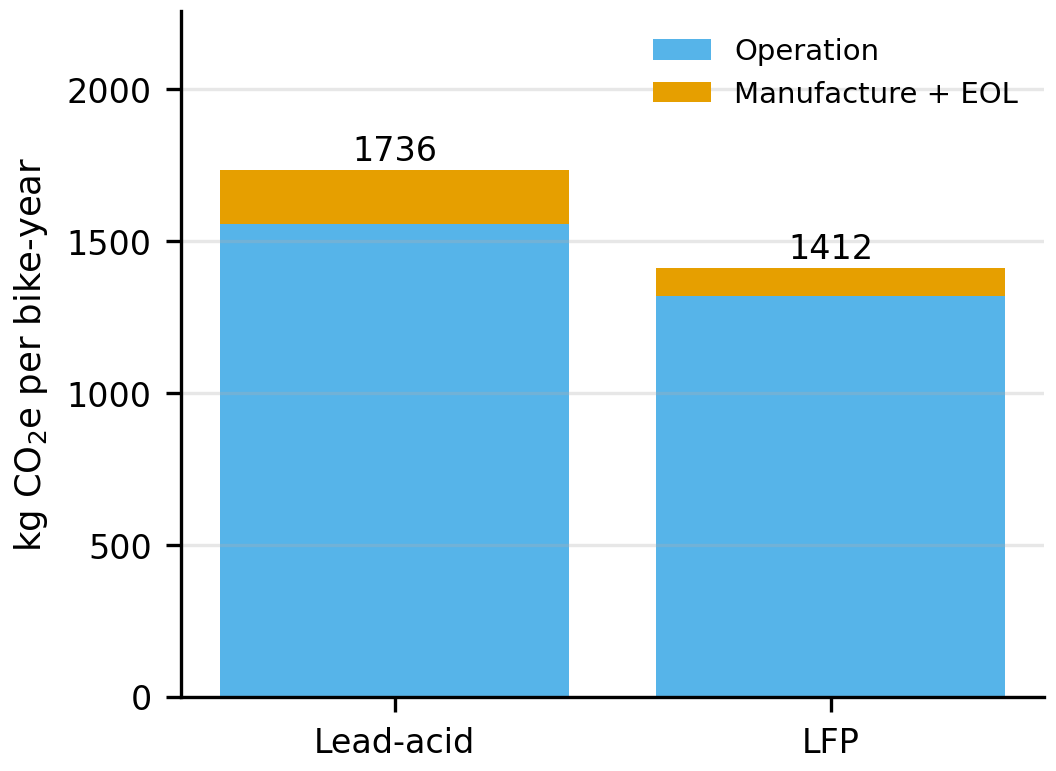
\includegraphics[width=0.45\textwidth]{fig5_co2_bike.png}\hfill
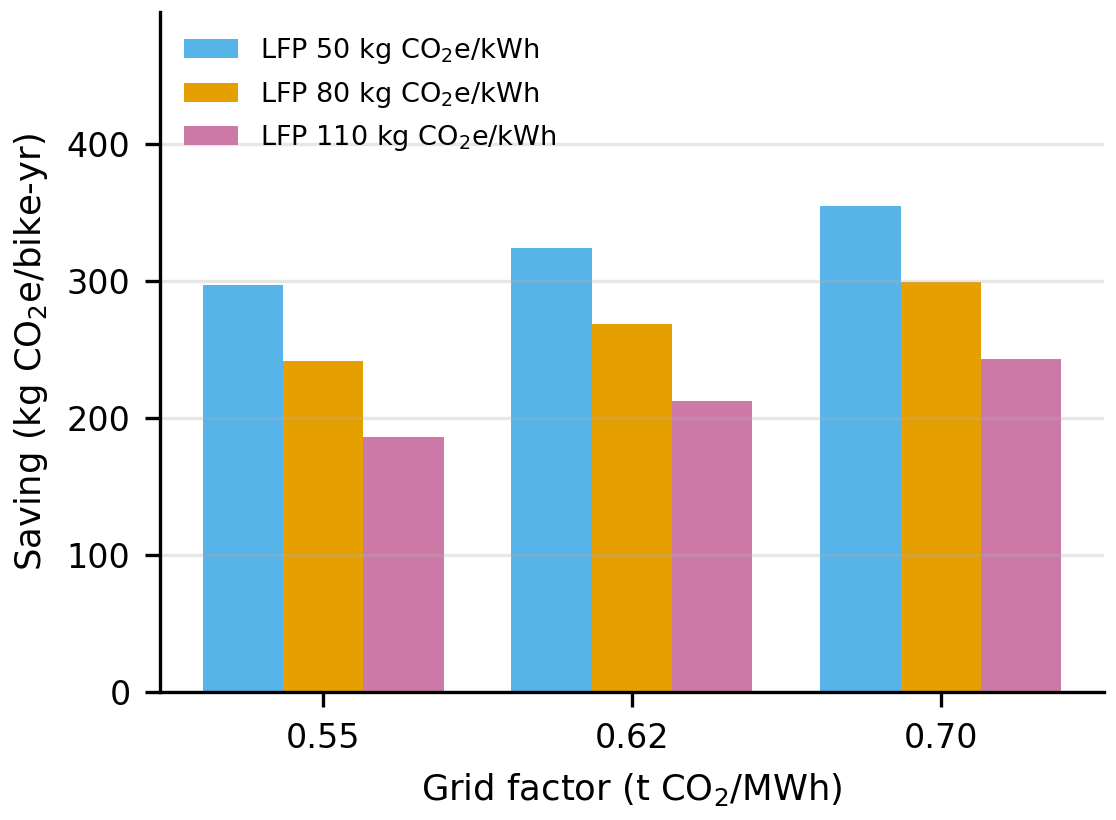
\includegraphics[width=0.45\textwidth]{fig7_co2_sensitivity.png}
\caption{Left: annual carbon footprint per bike. Right: per-bike saving from LFP for three LFP manufacturing footprints and three grid emission factors (\figref{co2sens}).}
\label{fig:co2}\label{fig:co2sens}
\end{figure}
The lead-acid fleet cycles \leadLow--\leadHigh{} kt of lead per year at 1.4 M bikes (Table~\ref{tab:lead}), or \leadBikeLow--\leadBikeHigh{} kg per bike-year; the upper value is close to the 167 kt reported by Pure Earth for recycling in the whole sector \cite{pureearth_smep}. Converted bikes need replacement so rarely that their lead flow in the model is negligible. Because LFP is dearer for the operator, conversion needs support: BDT \suppHalf{} billion over ten years for 50\% conversion and BDT \suppFull{} billion for full conversion (Table~\ref{tab:policy}, \figref{policy}). Per tonne of CO$_2$e saved the implied cost is BDT \abateCarbon{}, and per kilogram of lead kept out of recycling BDT \abateLead{} (BDT \abateLeadLow--\abateLeadHigh{} for 125 and 56 kg per set). These figures count only operator cost; they exclude the health benefits of less lead.
\begin{table}[t]
\caption{Lead throughput of the lead-acid fleet (kt Pb per year through replacement and recycling) at the survey replacement interval. 56 and 84 kg correspond to a four-battery set at 14 and 21 kg lead per battery; 125 kg is the Pure Earth figure.}
\label{tab:lead}
\centering\footnotesize
\begin{tabular}{lrr}
\hline
Lead per set & 1.4 M bikes & 3.0 M bikes \\
\hline
56 kg & 52 & 112 \\
84 kg & 79 & 168 \\
125 kg & 117 & 251 \\
\hline
\end{tabular}
\end{table}

\begin{table}[t]
\caption{Conversion scenarios for a 1.4 M-bike fleet (share moved from lead-acid to LFP). Lead flow assumes 84 kg Pb per lead-acid set (56--125 kg, Table~\ref{tab:lead}). Operator support is the 10-year cost difference that must be covered for LFP to match lead-acid.}
\label{tab:policy}
\centering\footnotesize
\setlength{\tabcolsep}{3pt}
\begin{tabular}{lrrrr}
\hline
Scenario & Share & CO$_2$e saved & Pb cycled & Support needed \\
 & (\%) & (Mt/yr) & (kt/yr) & ($10^9$ BDT) \\
\hline
S0 Business as usual & 0 & 0.00 & 79 & 0 \\
S1 Early adoption & 25 & 0.11 & 59 & 27 \\
S2 Targeted policy & 50 & 0.23 & 39 & 53 \\
S3 Full transition & 100 & 0.45 & 0 & 107 \\
\hline
\end{tabular}
\end{table}

\begin{figure}[t]
\centering
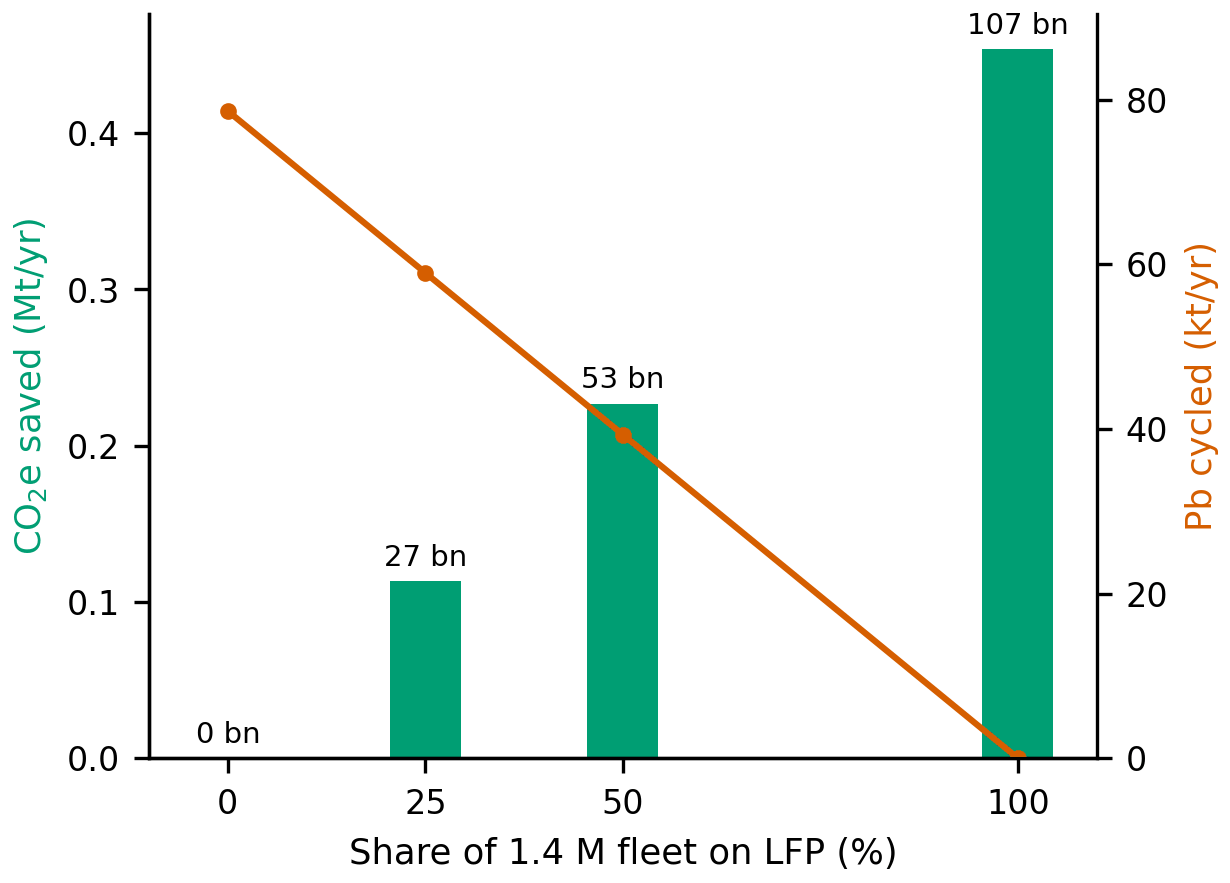
\includegraphics[width=0.5\textwidth]{fig6_policy.png}
\caption{Conversion scenarios: CO$_2$e saved (bars; labels give the operator support needed, $10^9$ BDT) and lead cycled through recycling (line) versus the share of the fleet on LFP.}
\label{fig:policy}
\end{figure}

\section{Discussion}
\label{sec:disc}
\subsection{What the survey changes}
Laboratory cycle lives favour LFP strongly, and a model built on them finds LFP cheaper over ten years (by BDT \litGap{}). The survey reverses this. A lead-acid set costs BDT \costMedLA{} and is expected to last \replMedLA{} months; an LFP set costs \costRatio{} times as much but lasts only \replMedLFP{}/\replMedLA{} $\approx$ 2.4 times as long, and it resells for \scrapLFP\% of its price against \scrapLA\% for lead-acid. Per month of use the capital cost net of resale is about BDT 940 for lead-acid and BDT 1{,}940 for LFP, while LFP's electricity saving (\egLA{} $-$ \egLFP{} kWh per day) is only about BDT 360 per month at BDT 11.36/kWh. For an operator who pays the purchase price, lead-acid is the cheaper choice at present prices, which is consistent with its dominance in the sample. The result depends on LFP prices of 2026, on the replacement intervals drivers expect, and on five LFP respondents.

\subsection{What would make lithium replace lead}
Break-even requires either a lower LFP price (BDT \beP{} at the surveyed life, \bePpct\% below the median), a much longer life (\beL{} months at the surveyed price), or a combination (\figref{breakeven}). The tornado chart shows that the main uncertainties are the real life of lead-acid and of LFP sets and the LFP price, all of which can be pinned down by following drivers over time. The conclusion also changes if lead-acid sets fail faster than the survey median (8 months would roughly equalise the two), for instance under heavier loads or hotter batteries. For LFP to win without a price fall, operators would need a way to recover its higher resale value or spread its cost, for example leasing or battery swapping.

\subsection{Temperature: what matters and what does not}
Regional temperature does \emph{not} separate Khulna, Chuadanga and Rajshahi: mean battery temperatures differ by \Tspread\,$^\circ$C and the ranking is identical. Temperature acts through the seasonal cycle, heat waves and above all the battery's rise above ambient: moving it from 0 to 10\,$^\circ$C cuts lead-acid life from 23.8 to 12.5 months and LFP life from 51.6 to 35.3 months (Table~\ref{tab:scen}), but both chemistries are affected, so the cost ranking does not change. Heat-wave days age lead-acid faster (\heatLA{} times) than LFP (\heatLFP{} times). Measuring pack temperature in service is a higher priority than adding weather stations.

\subsection{Carbon: a smaller prize than lead, but robust}
A full switch saves about \fleetA{} Mt CO$_2$e per year at 1.4 M bikes, and the per-bike saving stays between \sensMin{} and \sensMax{} kg across the tested manufacturing footprints and grid factors. As the grid decarbonises the operational saving falls while the embodied saving remains. At BDT \abateCarbon{} per tonne CO$_2$e the carbon case alone is an expensive route to emission cuts; the case for LFP rests mainly on lead.

\subsection{Lead, workers and public health}
Used lead-acid batteries are collected, broken open and their lead plates smelted, often by hand and close to homes and farmland. Pure Earth describes informal recycling that contaminates and poisons workers and nearby residents \cite{pureearth_smep}, and ESDO identifies it as a primary contributor to lead-pollution hotspots \cite{esdo2021}. The IEDCR bulletin reports that about 36 million children (60\%) are poisoned by lead, that market screening in Dhaka, Rajshahi, Khulna and Barishal found 24\% of 197 consumer samples above reference lead levels, and that home assessments in 47 Khulna households found high lead in metal and ceramic cookware and toys \cite{das2026}. The World Health Organization notes that no safe level of lead exposure is known \cite{who_lead}. Remediation helps only partly: soil lead fell 96\% at an abandoned Savar site while child blood lead fell 35\% \cite{chowdhury2021}; the IEDCR bulletin reports a 20\% fall at Mirzapur, where hotspot soil dropped from about 100{,}000 ppm to 60--100 ppm \cite{das2026}; and a Tangail study reports 22\% \cite{eos2026}. Because blood lead falls much less than soil lead, other sources persist, so removing the source of new contamination is as important as cleaning old sites. Only 30\% of ULAB recycling is reported to be formal \cite{fe2024}, and UNCTAD estimates that about 80\% is informal and that 15--20\% of the lead recycled informally is released to the environment \cite{unctad_smep}. If the sixteen Powder users also run lead-based batteries, 88\% of the surveyed drivers do.

Our model supplies the \emph{quantity} side: LFP conversion removes \leadLow--\leadHigh{} kt of lead per year from the recycling stream at 1.4 M bikes (\figref{lead}), at an implied operator cost of BDT \abateLeadLow--\abateLeadHigh{} per kg of lead. It does not estimate how much of that lead would reach people; that needs emission and exposure data that do not yet exist, and other sources (paint, spices, cookware) also contribute.
\begin{figure}[t]
\centering
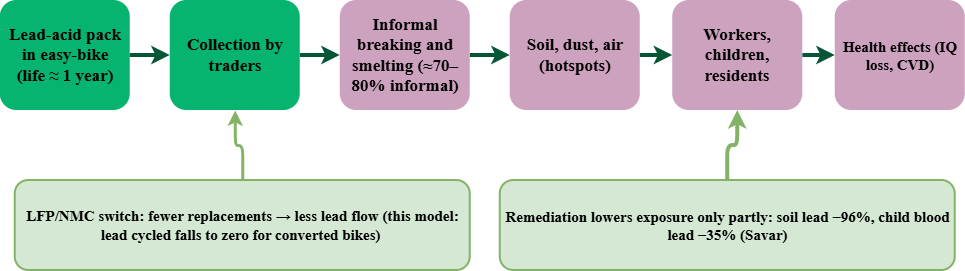
\includegraphics[width=0.9\textwidth]{fig_lead.png}
\caption{Pathway from lead-acid easy-bike batteries to exposure (schematic) and the point where an LFP switch acts; remediation figures from \cite{chowdhury2021}.}
\label{fig:lead}
\end{figure}

\subsection{Policy implications}
(i) \emph{Price and finance}: the BDT \premium{} premium and the BDT \gapLFP{} ten-year gap are barriers; leasing, pay-as-you-go and battery-swap schemes, or an import-duty cut that brings the LFP set below about BDT \beP{}, would close it. (ii) \emph{Support sized to the benefit}: full conversion of 1.4 M bikes needs about BDT \suppFull{} billion of support over ten years (Table~\ref{tab:policy}); this should be weighed against the health cost of lead, which is not in the model. (iii) \emph{ULAB regulation}: informal recycling is the main lead pathway, so licensed collection is a precondition for any lead benefit; the 2021 Hazardous Waste (e-waste) Management Rules reportedly cover household but not e-rickshaw lead batteries \cite{smep2024}. (iv) \emph{Lithium end of life}: a collection and recycling route must exist before volumes grow.

\subsection{Limitations}
\label{sec:limits}
\begin{itemize}
\item \textbf{Small convenience survey.} \nSurvey{} drivers, non-random, in the Khulna region; the LFP group has five respondents and four replacement answers, and these are expectations, not observed lifetimes. Several late-October entries have near-identical values, suggesting batch collection; excluding the ten from 27 October changes the lead-acid median from \replMedLA{} to \replLAnobatch{} months. \todo{[Insert survey locations and ethics statement.]}
\item \textbf{Calibration absorbs unknowns.} The fitted cycle lives (\NcalLA{} and \NcalLFP{}) also absorb operating days (not asked), charging practice and battery quality, and are not laboratory cycle lives.
\item \textbf{Equal pack size.} LFP capacity was not reported; it is set equal to the lead-acid Ah, and the LFP price is the median of sets of unknown capacity.
\item \textbf{Powder and charging cost.} Powder batteries (\nPW{} drivers) are not modelled because their chemistry is unconfirmed, and the charging-cost answers could not be pooled (per-charge, per-month and unspecified bases), so the tariff is taken from the BERC order and a hub-fee check.
\item \textbf{Energy use is from the literature}, not metered; the 52--88 Wh/km range is tested. The lead-acid pack runs above 80\% DoD at the survey distance.
\item \textbf{Cycle-limited life.} Calendar ageing is not modelled, and the LFP interval is an expectation.
\item \textbf{Vendor-level capacity curves, monthly temperature and an assumed battery temperature rise} (0--10\,$^\circ$C tested); hourly data would capture daily peaks.
\item \textbf{Scope.} NMC is not modelled because the survey contains no NMC users. Fire safety, weight and import dependence are not modelled, and lead flow is not exposure.
\item \textbf{Fleet size and tariff.} Fleet estimates range from 0.5 M autorickshaws to 4 M three-wheelers \cite{clean2024,pureearth_smep,unctad_smep}; the 3.0 M-bike results are an upper bound. The BDT 11.36/kWh rate is from press reports of the June 2026 BERC order \cite{berc2026fe,fenews2026}; tariffs of 7.70--16.24 change the gap by less than 15\%.
\end{itemize}

\section{Conclusion}
\label{sec:concl}
Using drivers' own prices, replacement intervals, resale values and daily distance from a survey of \nSurvey{} easy-bike drivers, together with NASA POWER temperature, we find that LFP is not yet the cheaper battery for the operator. At survey values a lead-acid set (BDT \costMedLA{}, \replMedLA{} months) costs BDT \tcoLA{} over ten years and an LFP set (BDT \costMedLFP{}, \replMedLFP{} months) BDT \tcoLFP{}, BDT \gapLFP{} (\gapPct\%) more, although laboratory cycle lives would suggest LFP is BDT \litGap{} cheaper. LFP matches lead-acid at a set price of about BDT \beP{} or a life of about \beL{} months. LFP still draws \gridratio\% less grid electricity, saves about \saveBike{} kg CO$_2$e per bike-year (\fleetA{} Mt per year for 1.4 M bikes) and removes \leadLow--\leadHigh{} kt of lead per year from informal recycling, at an operator support of BDT \suppFull{} billion over ten years for full conversion. Site temperature, which differs by only \Tspread\,$^\circ$C across Khulna, Chuadanga and Rajshahi, does not change the ranking, while battery heating and heat waves shorten the life of both chemistries and of lead-acid most. The answer to when lithium replaces lead is therefore economic and financial rather than climatic: it requires a cheaper or longer-lasting LFP set, or support and financing that recognise its lead and carbon benefits. The study rests on a small convenience survey, with LFP results from five drivers, and should be repeated with metered operating data and a larger, randomised sample.

\section{Reproducibility}
\label{sec:repro}
The analysis runs in MATLAB R2024a with the files in the \texttt{matlab} folder: (1) \texttt{easybike\_survey} (survey tables and figures from \texttt{survey\_cleaned.csv}); (2) \texttt{easybike\_main} (model tables and figures); (3) \texttt{easybike\_co2} (carbon, lead and policy tables); (4) \texttt{easybike\_build\_simulink} (builds \texttt{easybike\_battery.slx} and verifies it against the analytic model); (5) \texttt{easybike\_check} (compares a user's \texttt{results\_summary.csv} with \texttt{expected\_results.csv}). All inputs live in \texttt{easybike\_params.m}, each tagged with its source; the survey-based inputs are computed from \texttt{survey\_cleaned.csv}. The tables and figures in this paper were generated by a Python implementation of the same equations, which reproduced an earlier MATLAB \texttt{results\_summary.csv} to 15 significant digits. \todo{[Run easybike\_main and easybike\_check in MATLAB with the survey parameters and confirm MATCH before submission.]}

\appendices
\section{Survey Data Handling}
\label{app:survey}
The cleaned data (\texttt{survey\_cleaned.csv}, 43 rows) keep one value per field in one unit. The rules applied, and the answers that needed interpretation, were:
\begin{itemize}
\item Bengali digits were converted to Western digits; ``k'' was read as thousands of taka (90k = BDT 90{,}000); ranges (for example 70--100 km, 12--24 months) were replaced by their mid-points.
\item ``Powder'' was entered by the surveyor as a separate battery type and is kept separate; it is not merged with lead-acid.
\item Purchase prices of BDT 60{,}000 or more were recorded for seven lead-based respondents; they were kept and the median is used.
\item Capacity per battery was reported by only five respondents (120, 120, 160, 180 and 30 Ah). The 30 Ah answer accompanies a six-battery, 72 V set and was treated as a charger current, not a battery capacity.
\item Charging-cost answers mix per-charge, per-month and unspecified bases and were not used.
\item Problem answers were grouped into six categories; the two Bengali phrasings of ``low charge'' were merged.
\end{itemize}

\section{Simulink Verification}
\label{app:sim}
The Simulink model was verified against the analytic code in a run of twelve cases (three chemistries at 15, 25, 35 and 45\,$^\circ$C, earlier parameter set); efficiency, end-of-day SOC and range were identical to the printed precision in every case. Table~\ref{tab:sim} gives the analytic values for the survey parameter set that the final run must reproduce. \todo{[Re-run easybike\_build\_simulink with the survey parameters, confirm PASS and add the Simulink columns.]}
\begin{table}[t]
\caption{Analytic reference values for the survey parameter set (output of \texttt{easybike\_discharge}): discharge efficiency $\eta$, end-of-day SOC and range at four battery temperatures. The Simulink model must reproduce them to the printed precision (acceptance: 0.5 percentage points in $\eta$, 0.01 in SOC, 2\% in range).}
\label{tab:sim}
\centering\footnotesize
\begin{tabular}{lrrrr}
\hline
Battery & $T$ ($^\circ$C) & $\eta$ & SOC$_{end}$ & Range (km) \\
\hline
Lead-Acid & 15 & 0.8170 & 0.000 & 57.4 \\
Lead-Acid & 25 & 0.8803 & 0.083 & 66.3 \\
Lead-Acid & 35 & 0.9172 & 0.148 & 71.4 \\
Lead-Acid & 45 & 0.9406 & 0.182 & 74.4 \\
LFP & 15 & 0.9662 & 0.111 & 68.4 \\
LFP & 25 & 0.9747 & 0.172 & 73.4 \\
LFP & 35 & 0.9806 & 0.187 & 74.8 \\
LFP & 45 & 0.9849 & 0.196 & 75.6 \\
\hline
\end{tabular}
\end{table}


\section*{Data Availability}
The cleaned survey data (43 responses), the NASA POWER files (monthly T2M, 2024-01-01 to 2025-12-31, points 22.84$^\circ$N 89.57$^\circ$E, 23.64$^\circ$N 88.69$^\circ$E and 24.38$^\circ$N 88.60$^\circ$E), the MATLAB/Simulink code and all result tables will be made available in a public repository. \todo{[Add repository DOI.]}
\section*{Acknowledgment}
The author thanks \todo{[supervisor, institution and the drivers who answered the survey]}. In line with journal policy on generative AI, the author discloses that an AI assistant (Anthropic Claude) was used to help draft code, text and figures; the authors reviewed all content and are responsible for it. \todo{[Edit as the journal requires.]}
\bibliographystyle{ieeetr}
\bibliography{references}
\end{document}
